% !TEX root = main.tex
\section{Acceptance}
\label{sec:Acceptance}

\subsection{MC corrections}

\subsubsection{Truth matching of simulated candidates}

We use the \textsf{BackgroundCategory} tool to truth match our simulated candidates. 
Candidates with background category (\textsf{BKGCAT}) 20 or 50 are considered to be true signal. 
Background category 60 is more peculiar since it contains both badly reconstructed
signal candidates and ghost background.
This is due to the fact that the classification algorithms identifies all tracks 
for which less than $70\%$ of the reconstructed hits are matched to generated truth-level quantities as ghosts.
In particular for signal decays involving many tracks (as in our case),
this arbitrary cutoff is not $100\%$ efficient.
Moreover, the efficiency is expected to depend on the kinematics which would lead to a biased acceptance determination
if candidates with \textsf{BKGCAT}$=60$ would be removed. \\
We therefore include \textsf{BKGCAT}$=60$ and statistically subtract the ghost background by using the \textsf{sPlot} technique.
The \textsf{sWeights} are calculated from a fit to the reconstructed $B_s$ mass.  
The signal contribution is modeled as described in Sec.~\ref{subsec:signalModel} and the background with a polynomial.
The fit is performed simultaneously in two categories; the first includes events with \textsf{BKGCAT} = 20 or 50 and
the second events with \textsf{BKGCAT}  = 60.
To account for the different mass resolution we use a different $\sigma$ for each category,
while the mean and the tail parameters are shared between them. 
The background component is only included for the second category.
\\
A significant fraction of $8\%$ of the true signal candidates are classified as ghosts,
while only $20 \%$ of the events classified with \textsf{BKGCAT}$=60$ are indeed genuine ghosts.


%We repeat the efficiency determination with an alternative fit model to assign a systematic uncertainty.


\begin{figure}[h]
\centering
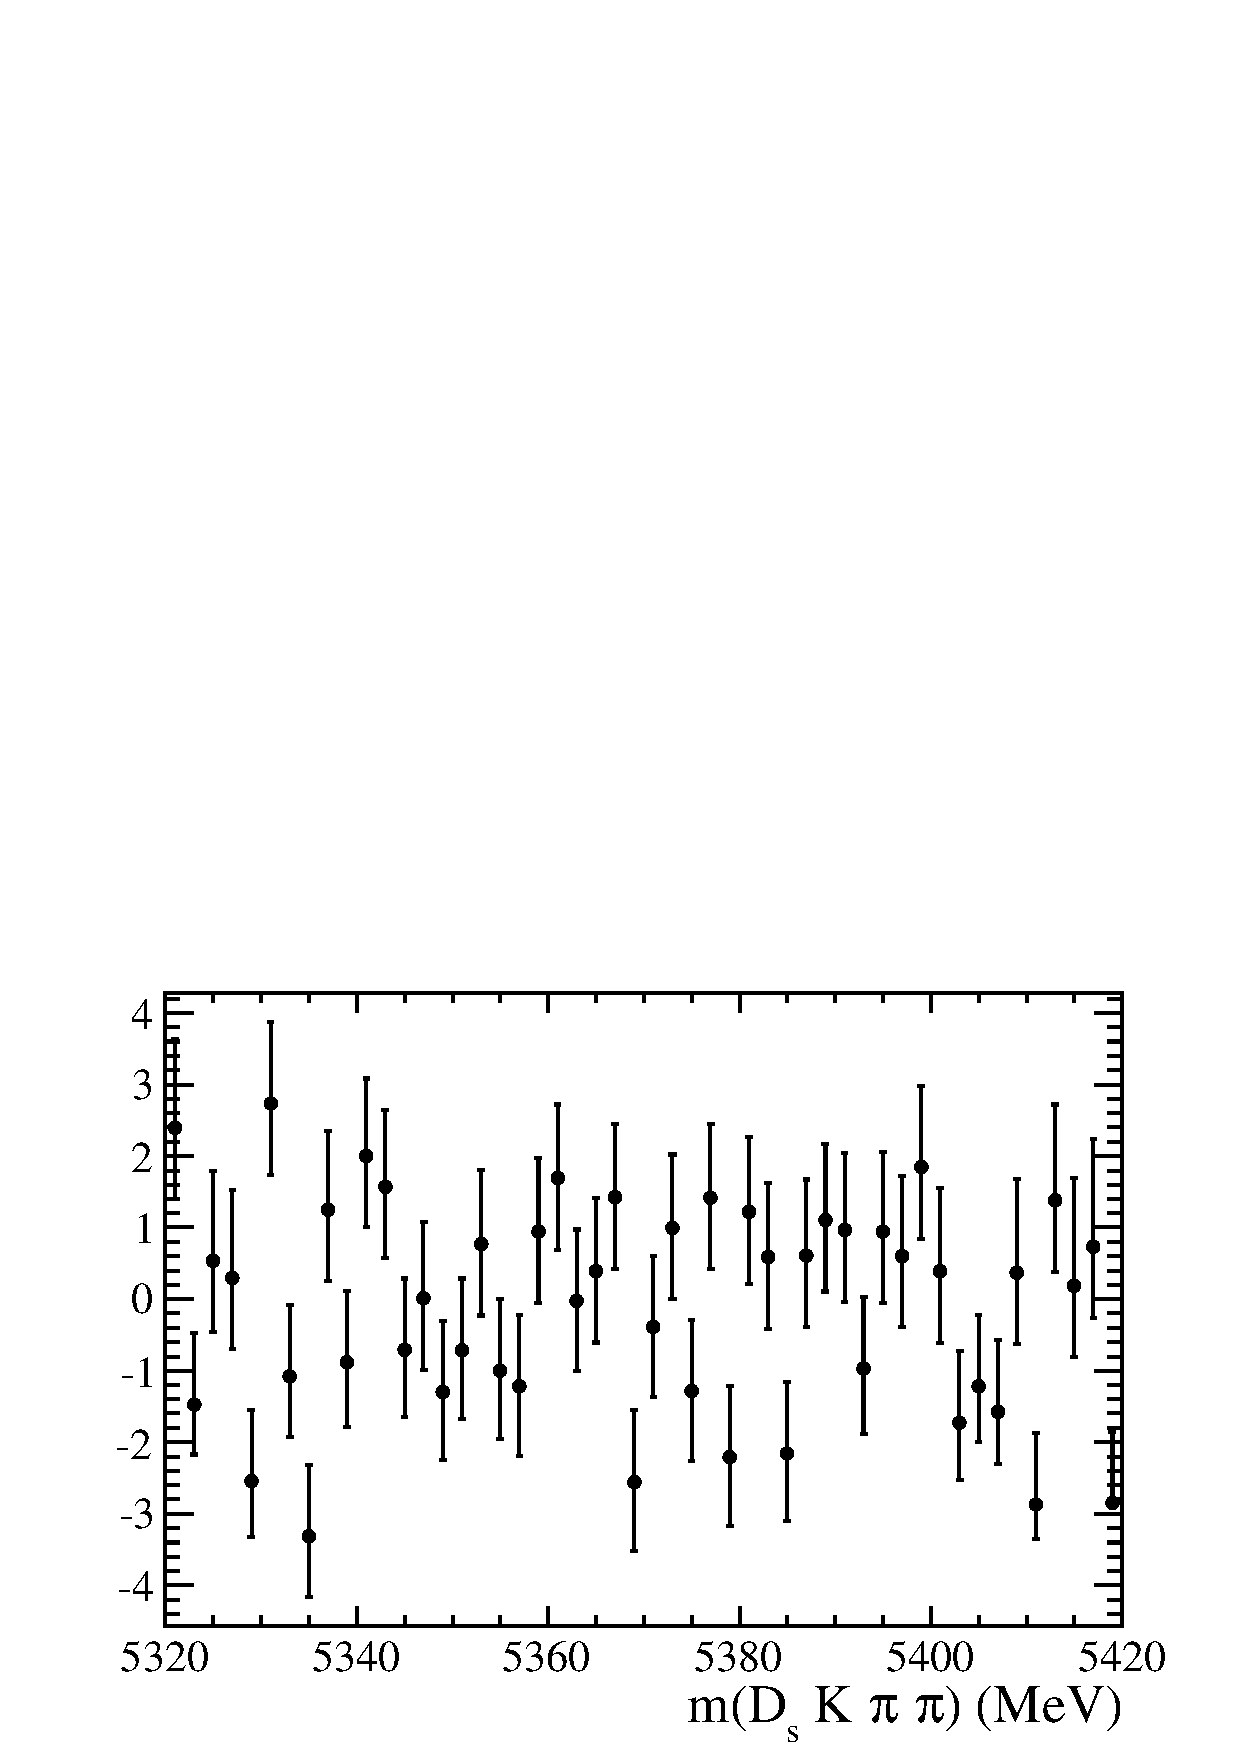
\includegraphics[height=!,width=0.4\textwidth]{figs/MassFit/signalMC_pull.pdf}
\includegraphics[height=!,width=0.4\textwidth]{figs/MassFit/signalMC_ghost_pull.pdf}

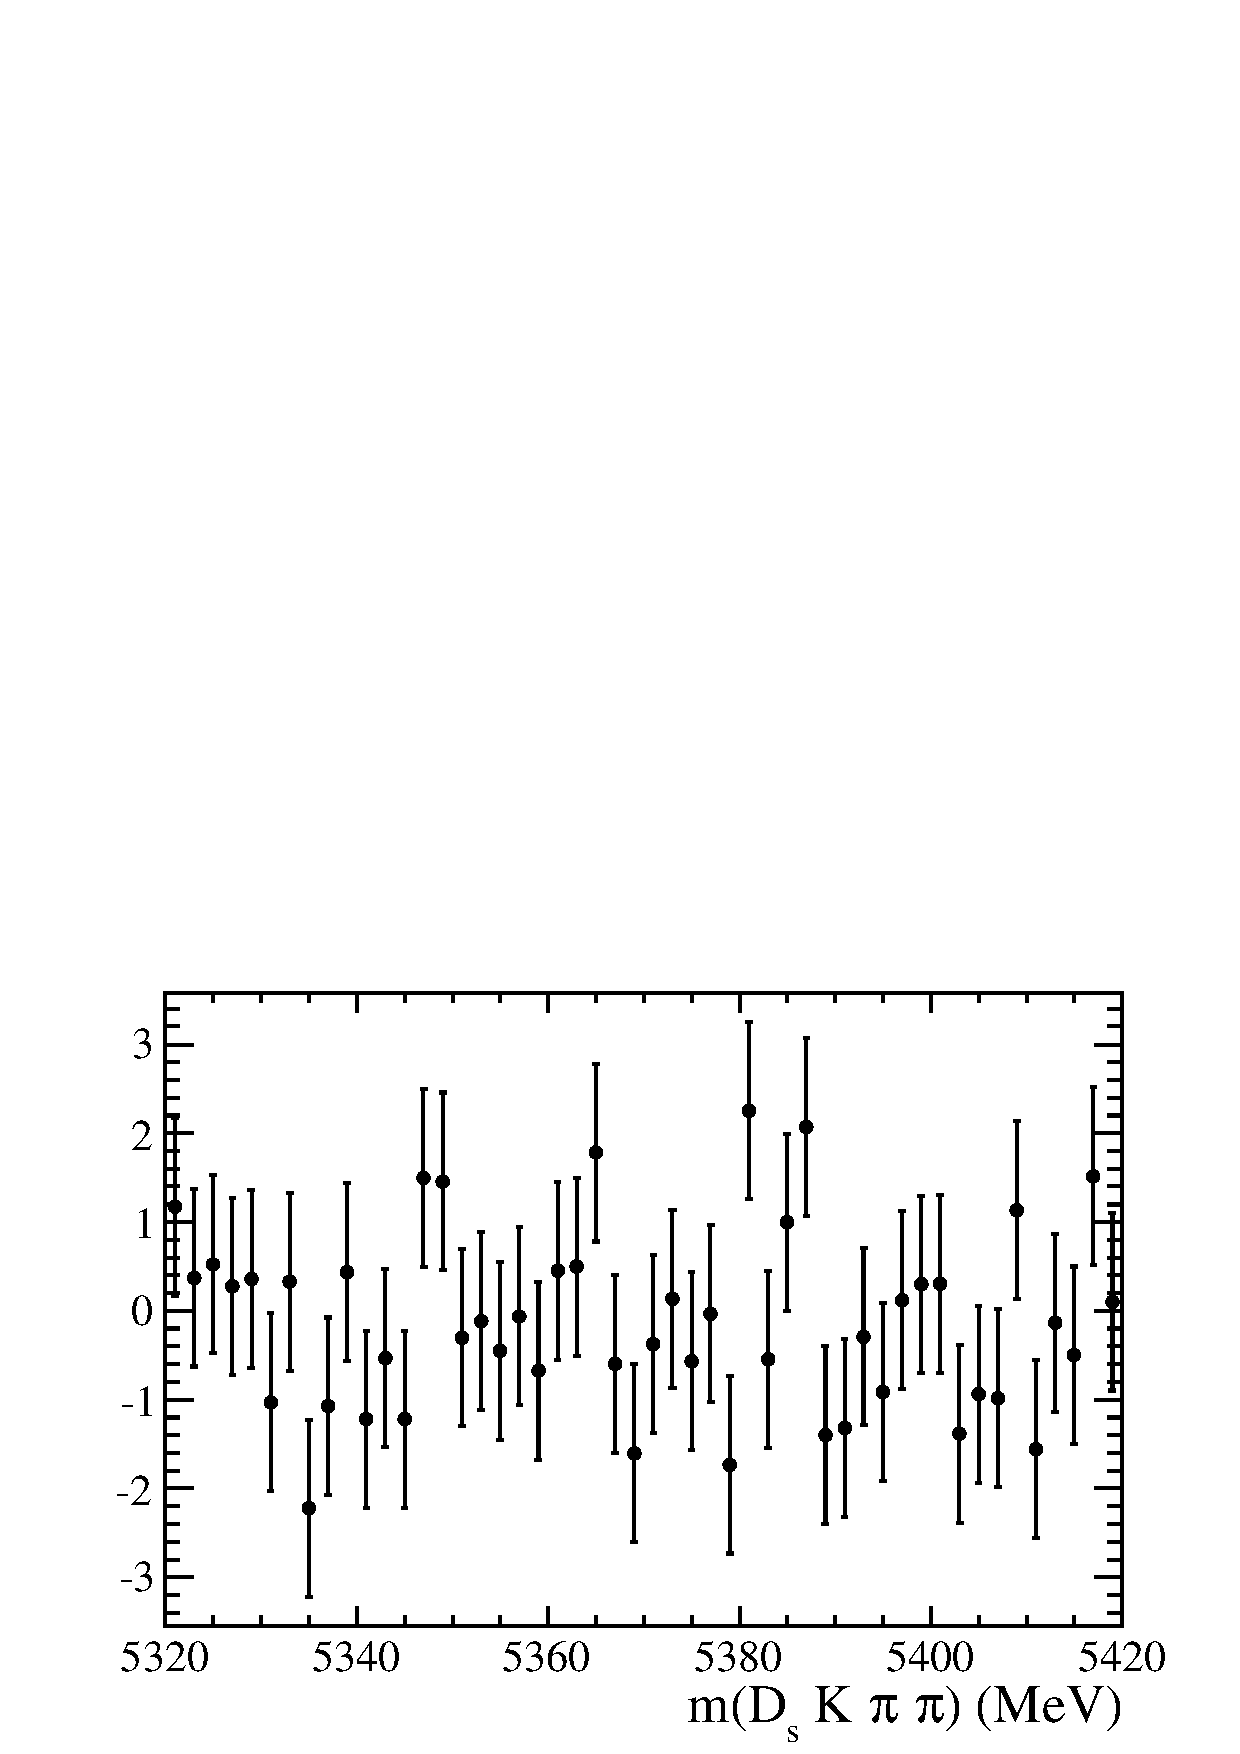
\includegraphics[height=!,width=0.4\textwidth]{figs/MassFit/normMC_pull.pdf}
\includegraphics[height=!,width=0.4\textwidth]{figs/MassFit/normMC_ghost_pull.pdf}

\caption{The reconstructed $B_s$ mass distribution for simulated $B_s \to D_s K \pi \pi$ (top) and $B_s \to D_s \pi \pi \pi$ (bottom) decays 
classified with \textsf{BKGCAT} = 20 or 50 (left) and \textsf{BKGCAT} = 60 (right) after the full selection. }
\label{fig:}
\end{figure}

%\clearpage
%\subsubsection{PID efficiencies}
%
%\begin{figure}[h]
%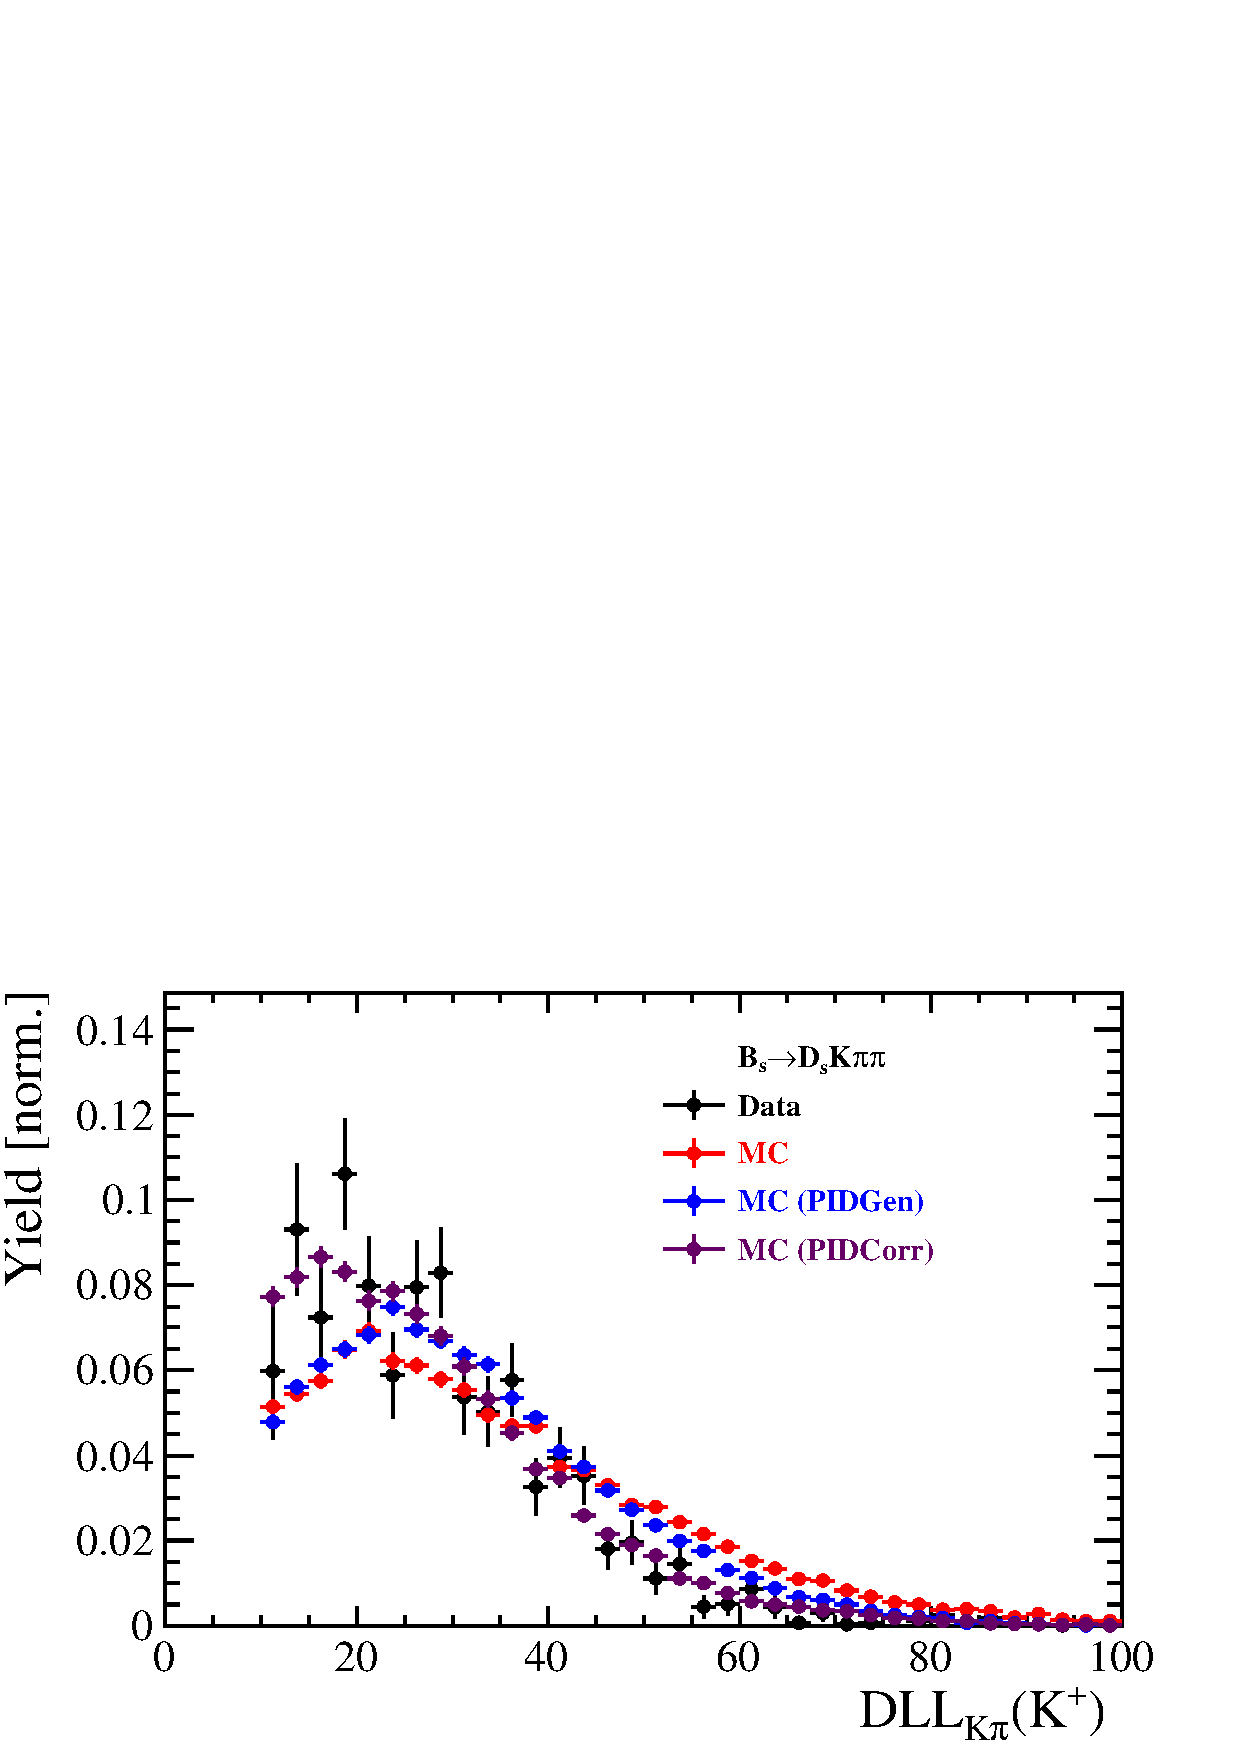
\includegraphics[height=!,width=0.32\textwidth]{figs/dataVsMC/signal_pid/PID_Ds2KKpi_1_K_plus_PIDK.pdf}
%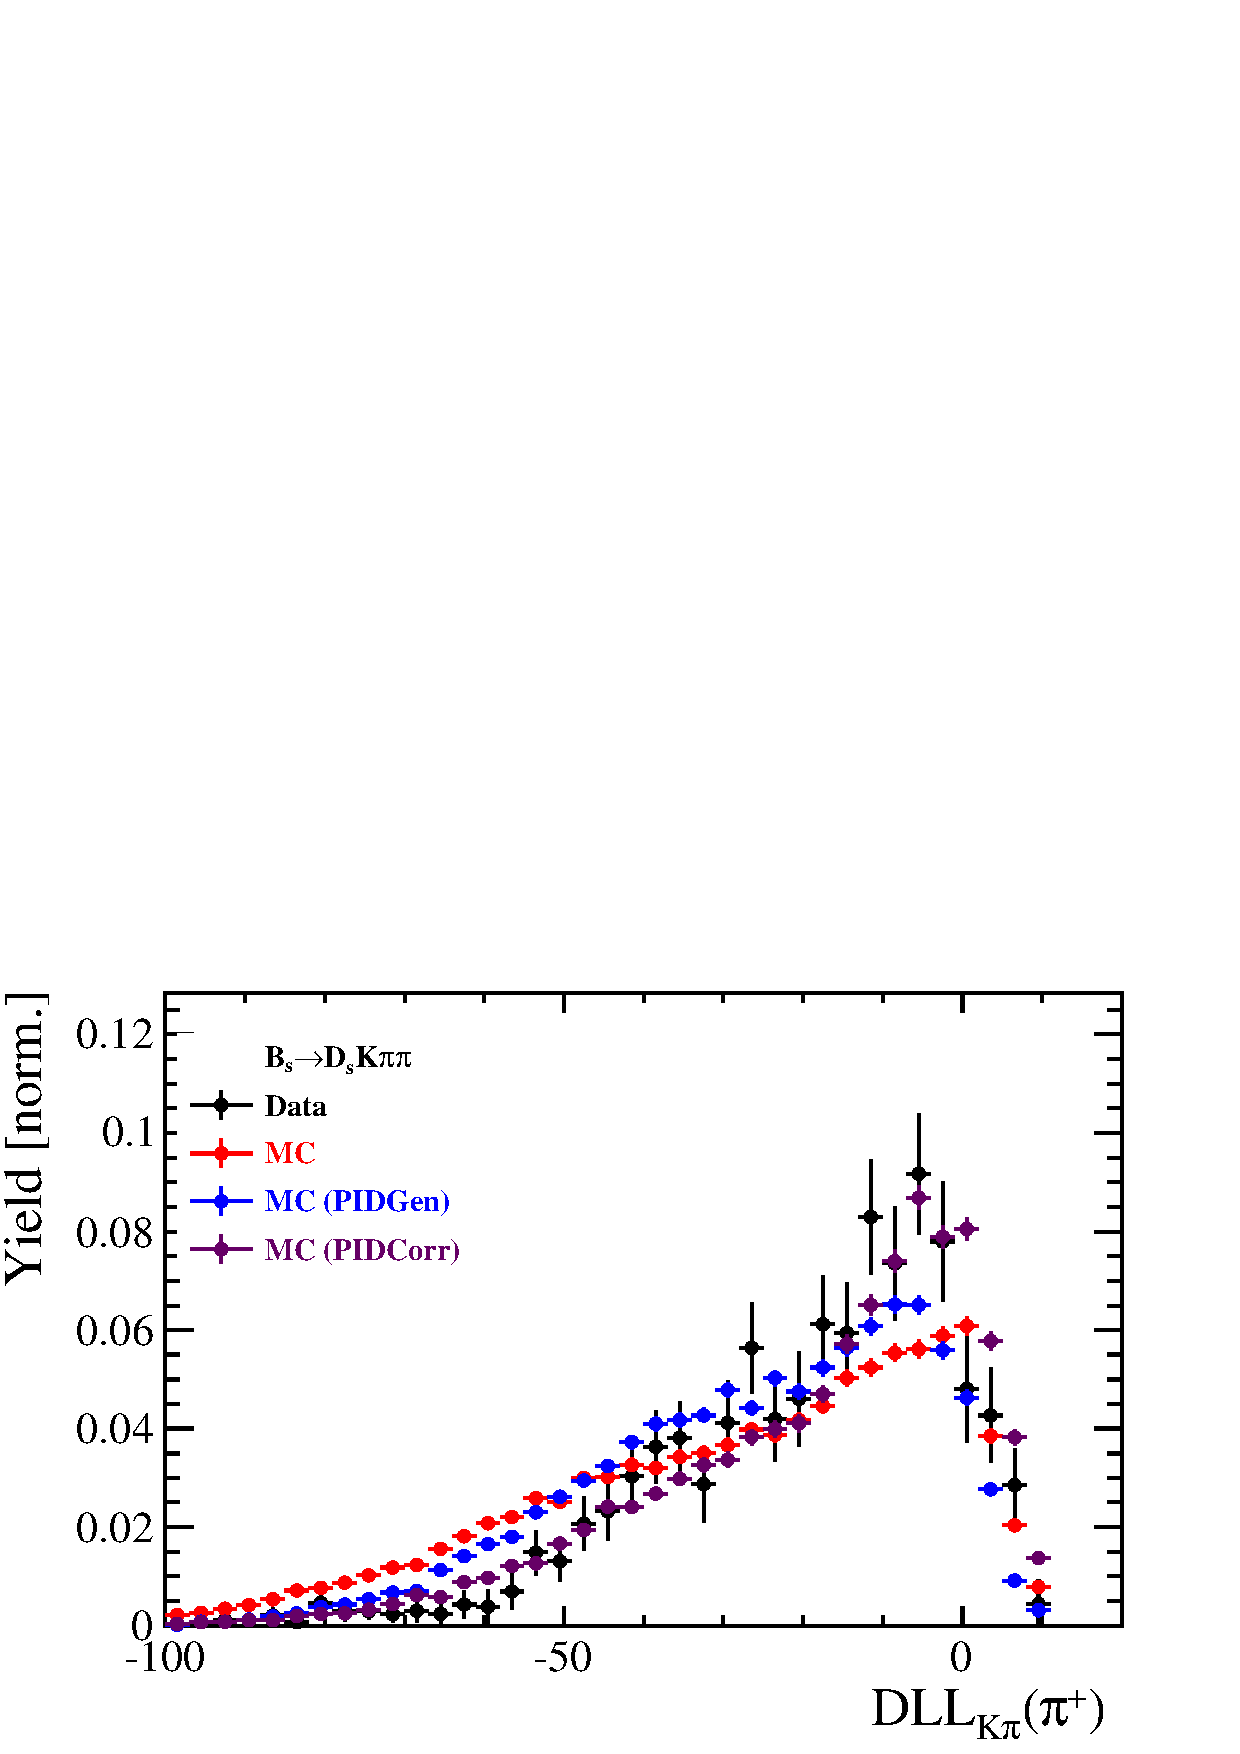
\includegraphics[height=!,width=0.32\textwidth]{figs/dataVsMC/signal_pid/PID_Ds2KKpi_1_pi_plus_PIDK.pdf}
%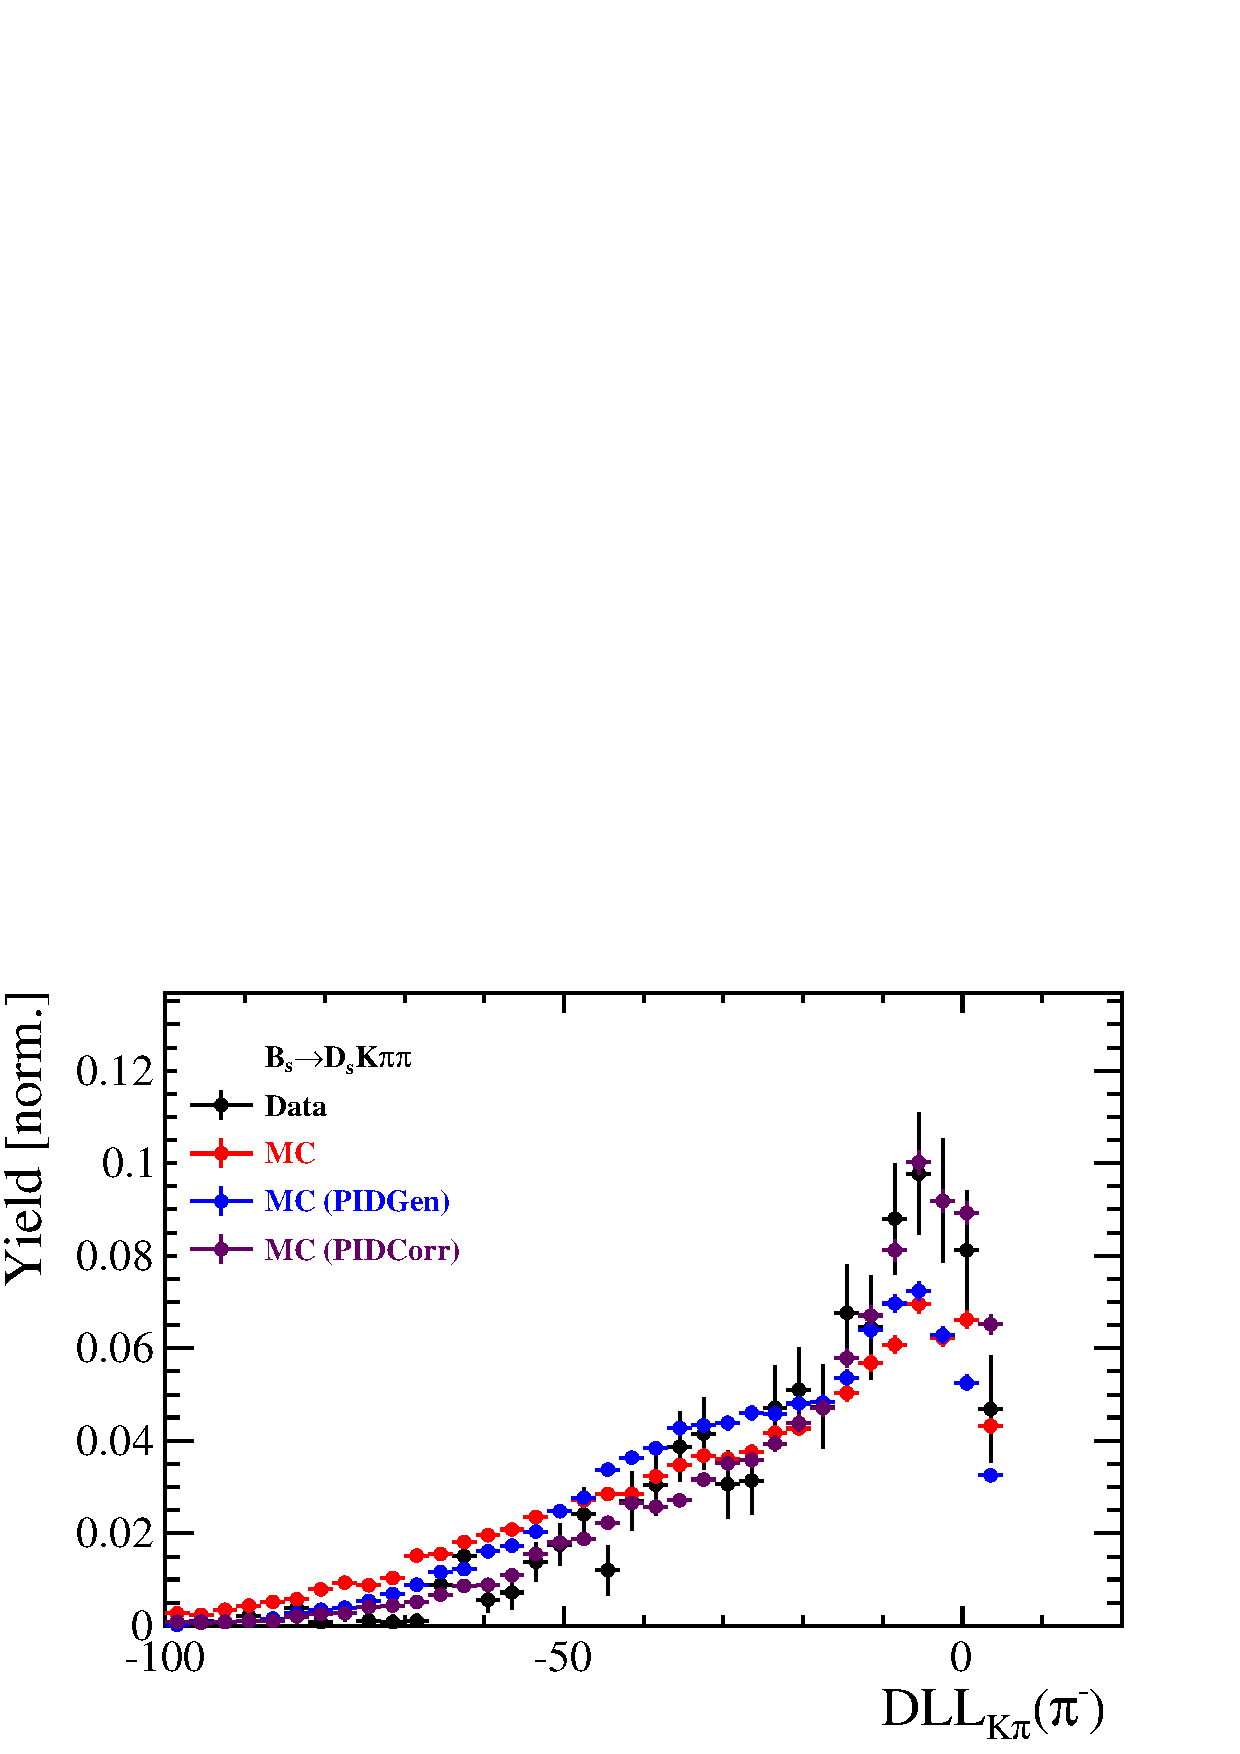
\includegraphics[height=!,width=0.32\textwidth]{figs/dataVsMC/signal_pid/PID_Ds2KKpi_1_pi_minus_PIDK.pdf}
%
%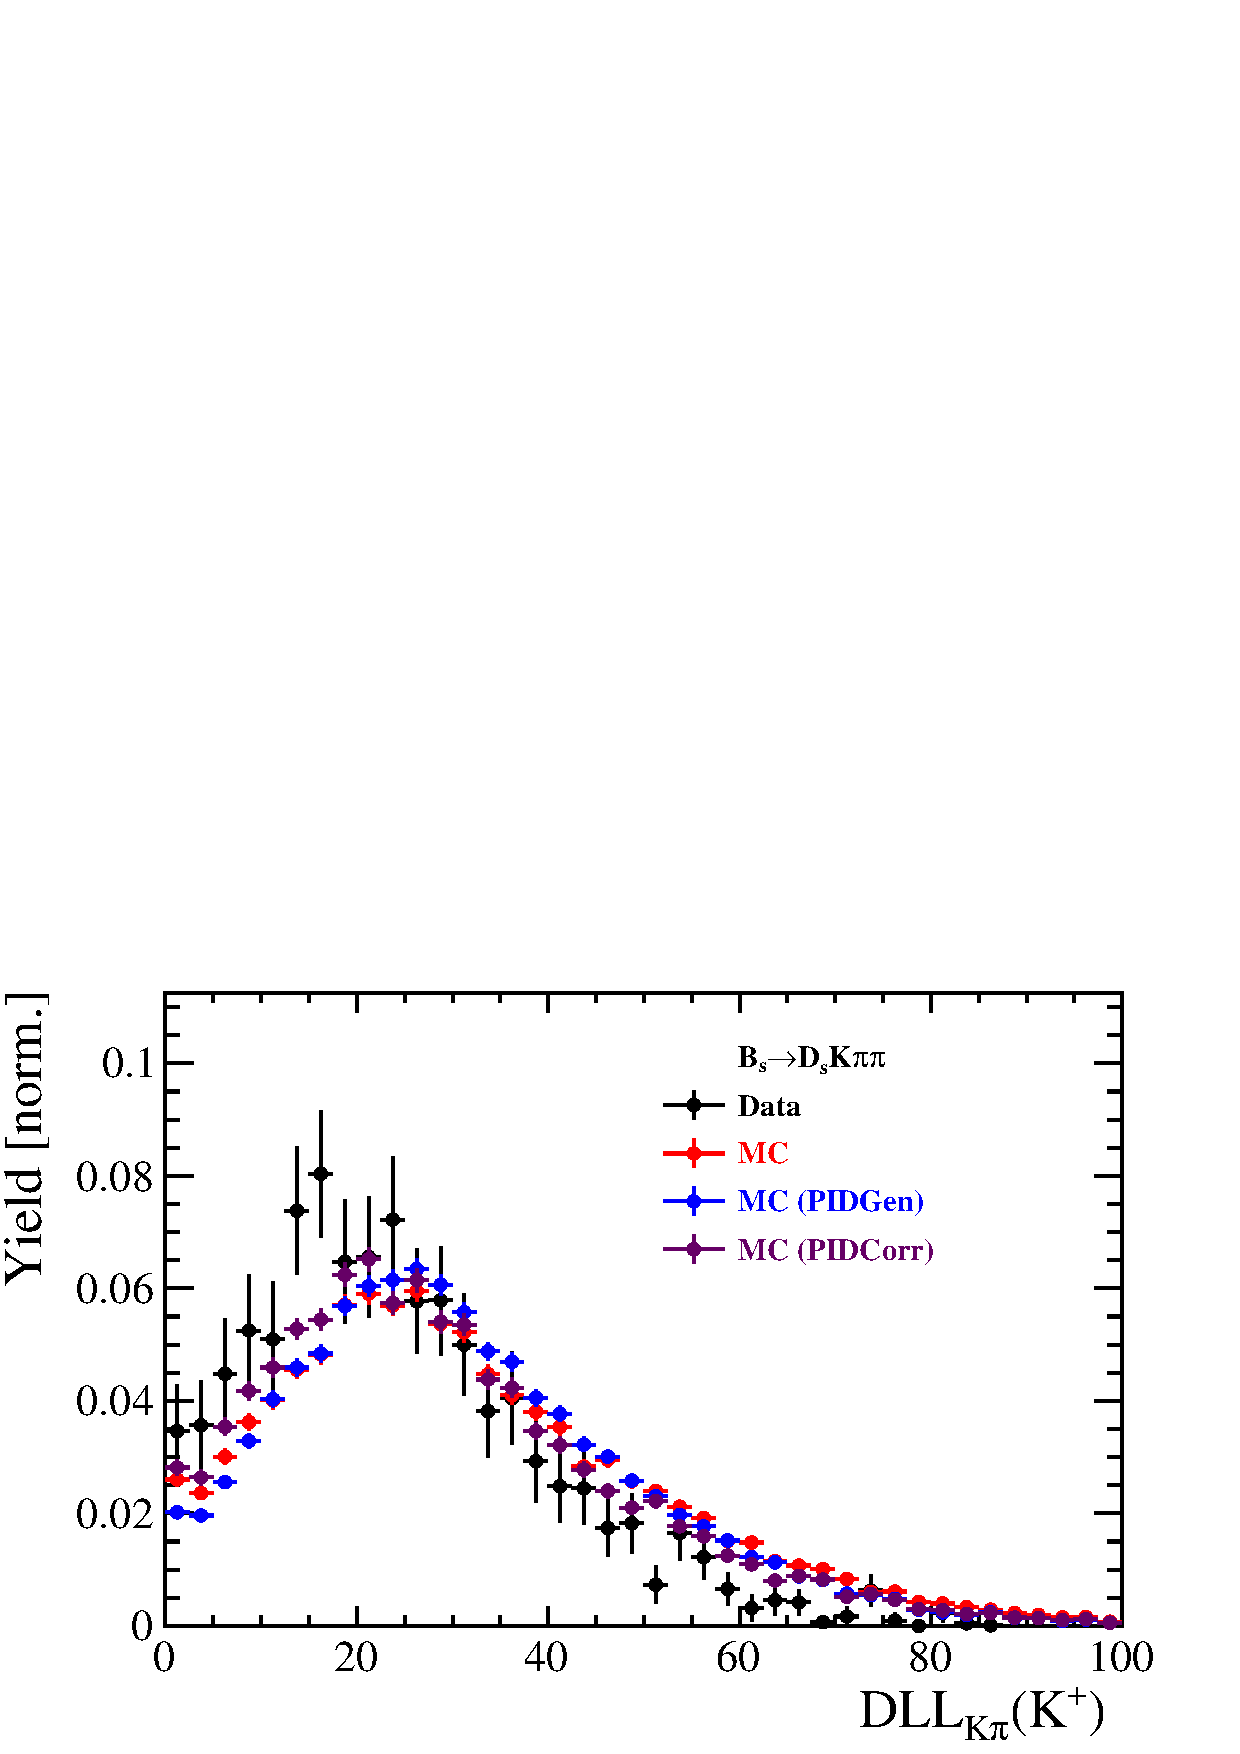
\includegraphics[height=!,width=0.32\textwidth]{figs/dataVsMC/signal_pid/PID_Ds2KKpi_1_K_plus_fromDs_PIDK.pdf}
%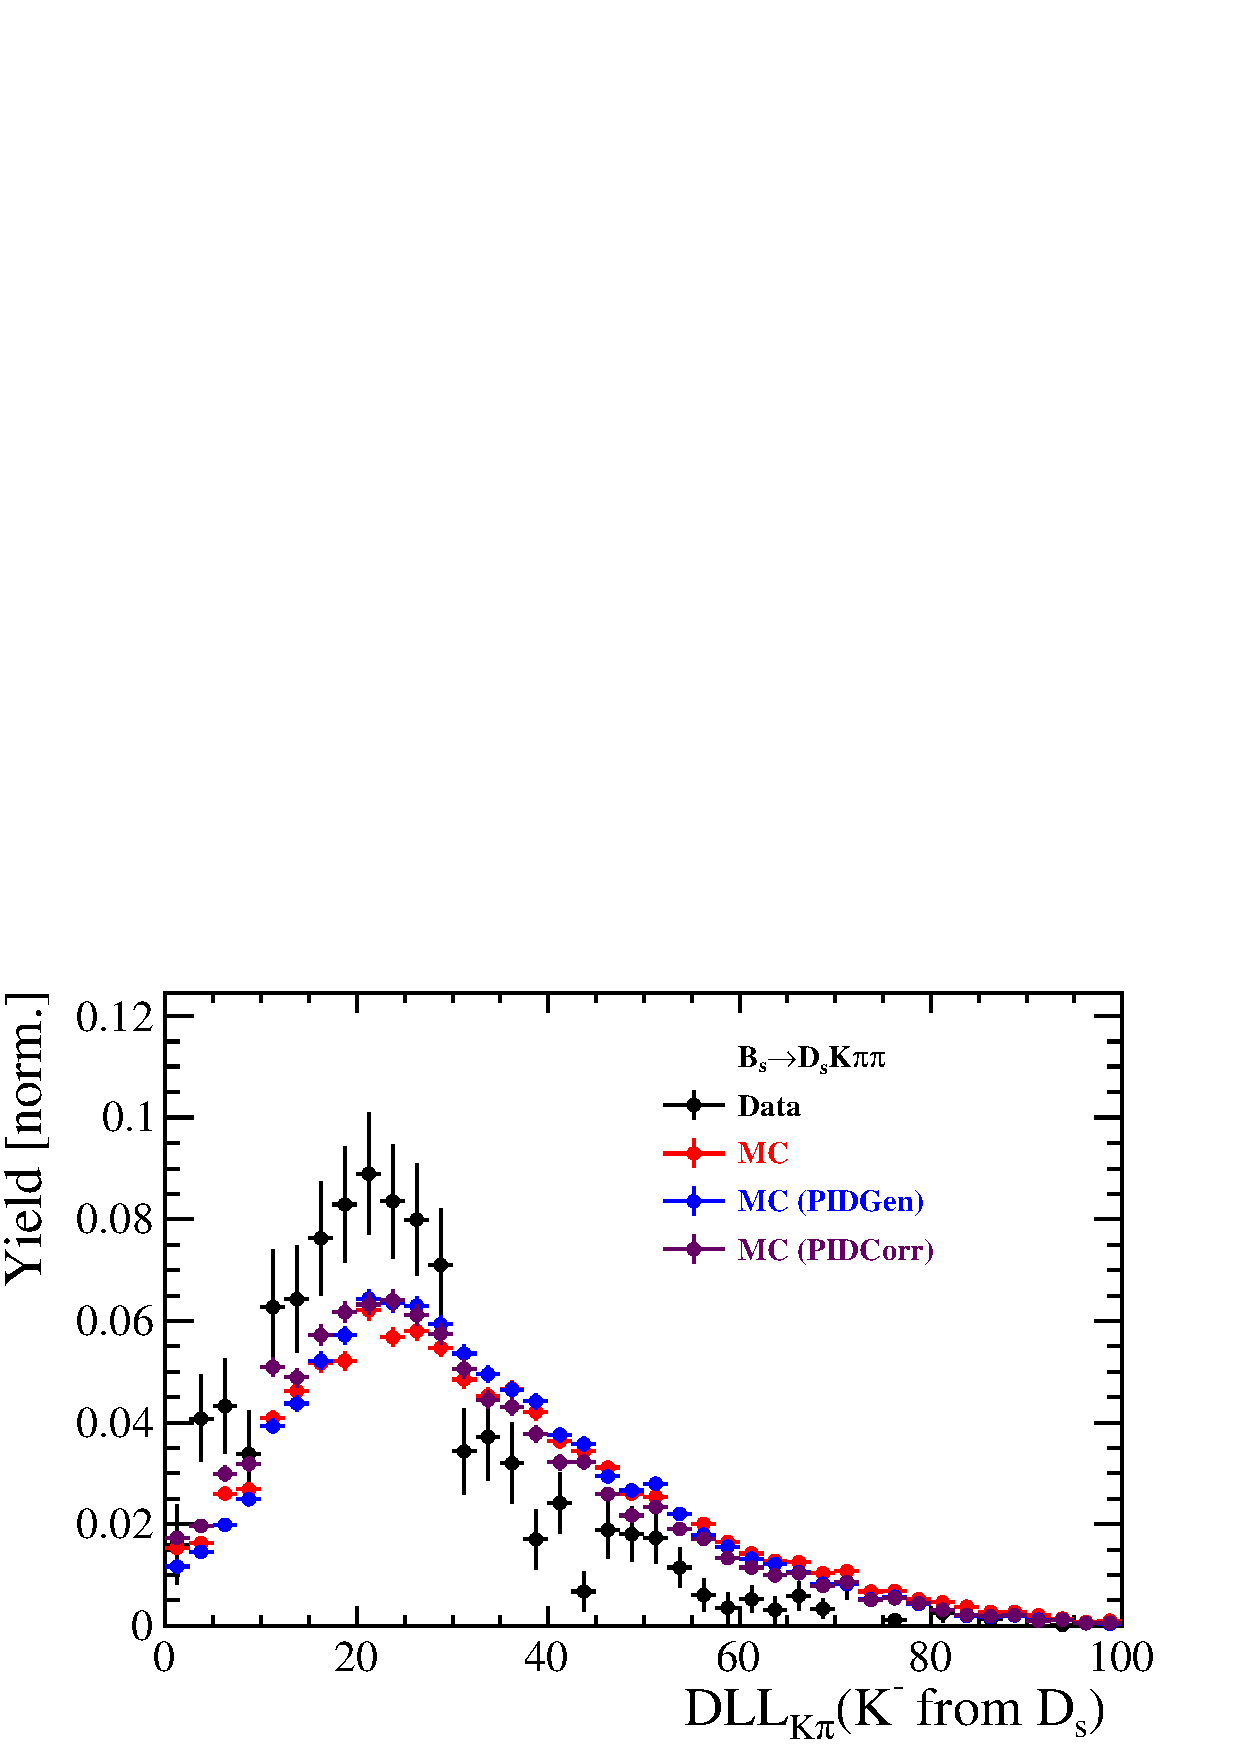
\includegraphics[height=!,width=0.32\textwidth]{figs/dataVsMC/signal_pid/PID_Ds2KKpi_1_K_minus_fromDs_PIDK.pdf}
%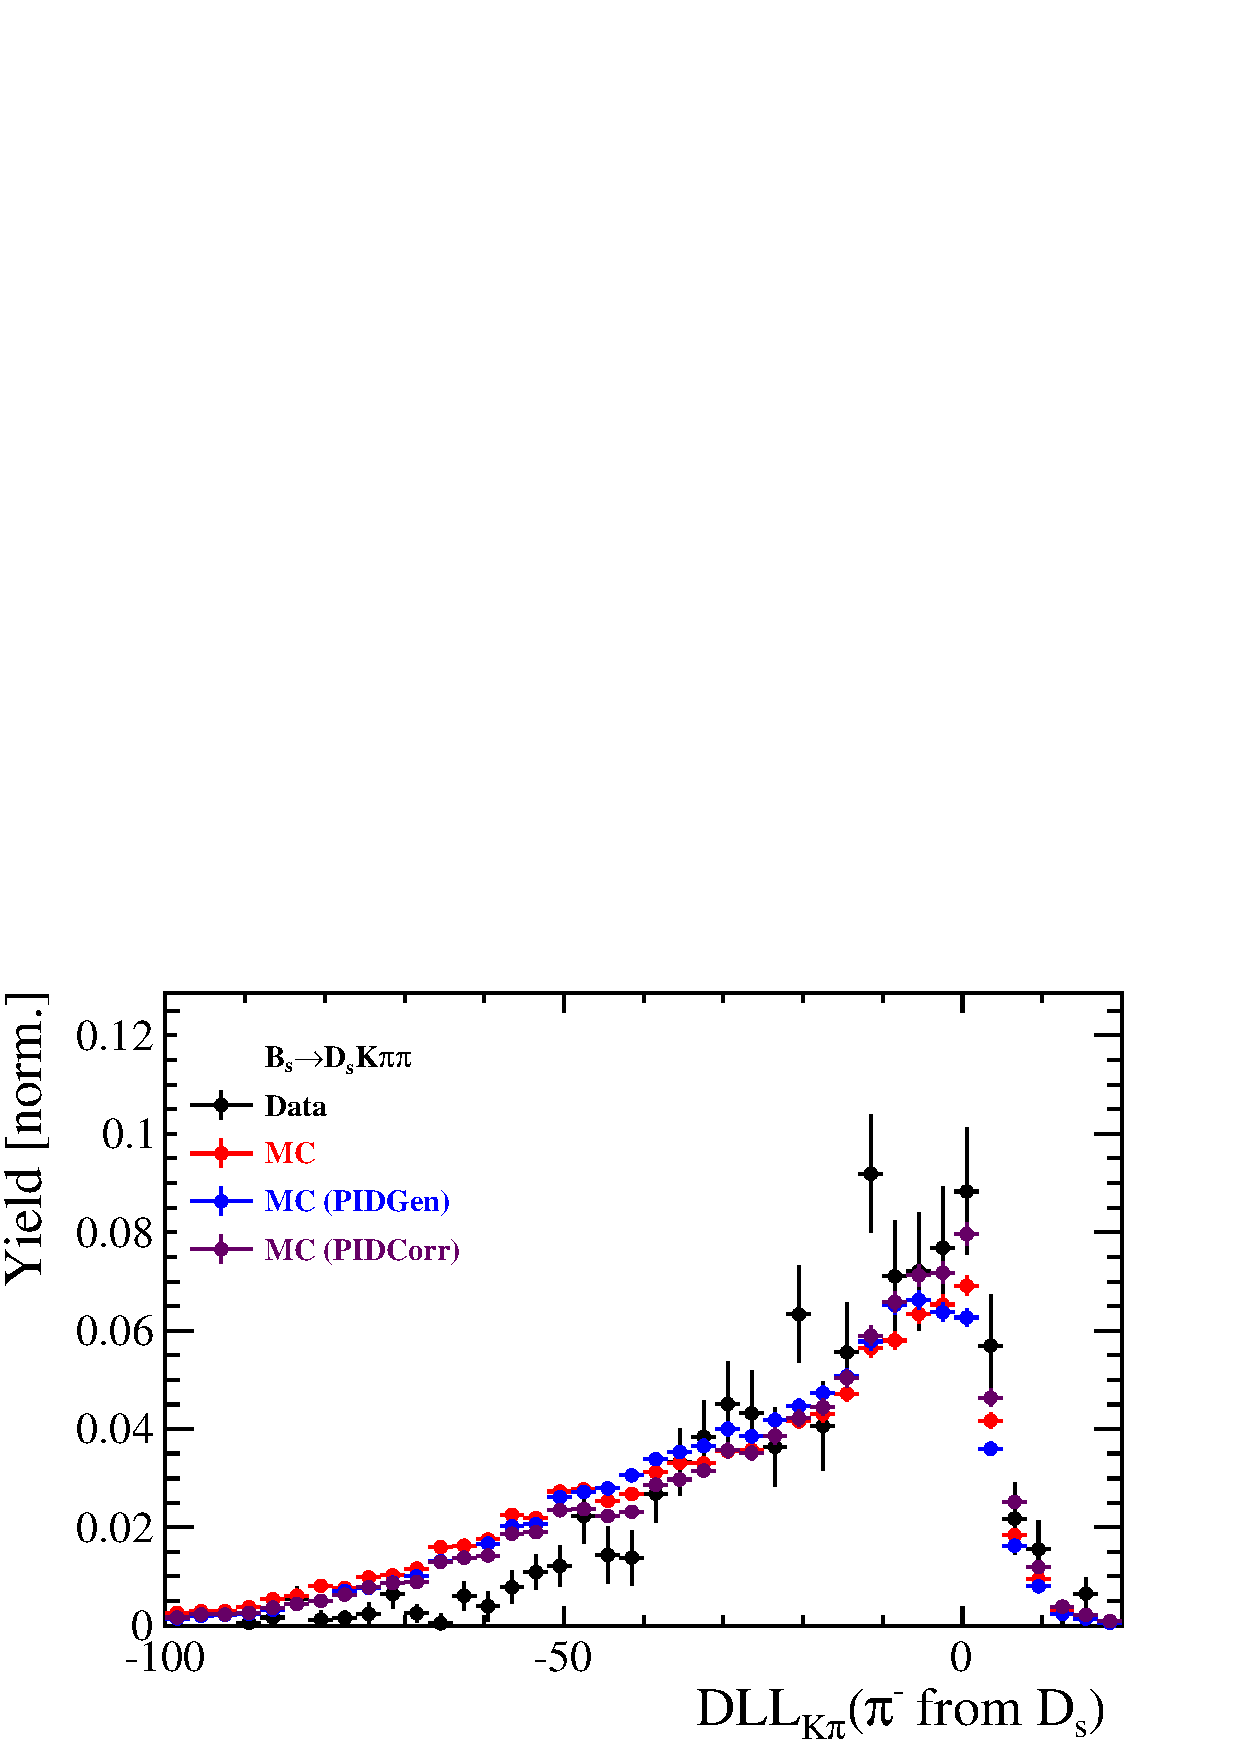
\includegraphics[height=!,width=0.32\textwidth]{figs/dataVsMC/signal_pid/PID_Ds2KKpi_1_pi_minus_fromDs_PIDK.pdf}
%\caption{}
%\label{fig:}
%\end{figure}
%
%\begin{figure}[h]
%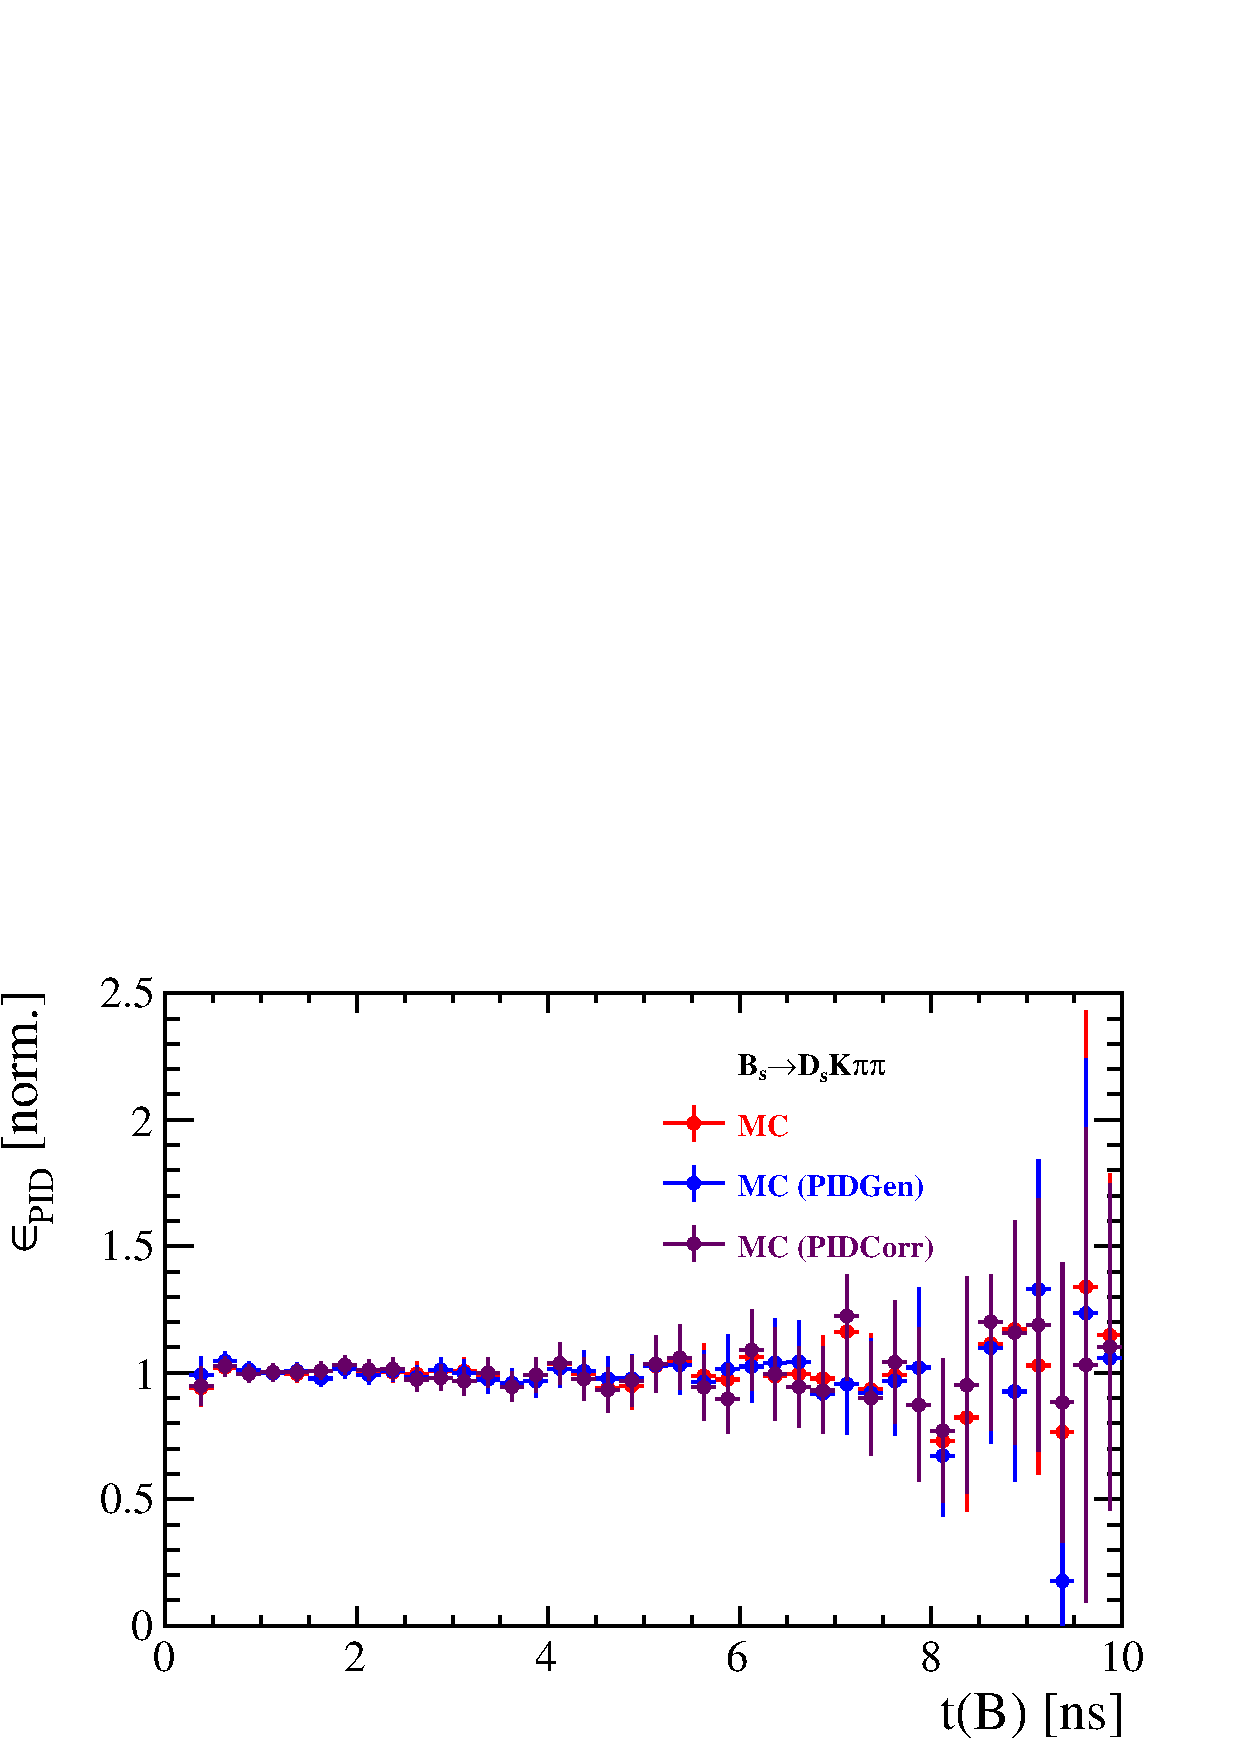
\includegraphics[height=!,width=0.32\textwidth]{figs/dataVsMC/signal_pid/eff_PID_Ds2KKpi_1_Bs_DTF_TAU.pdf}
%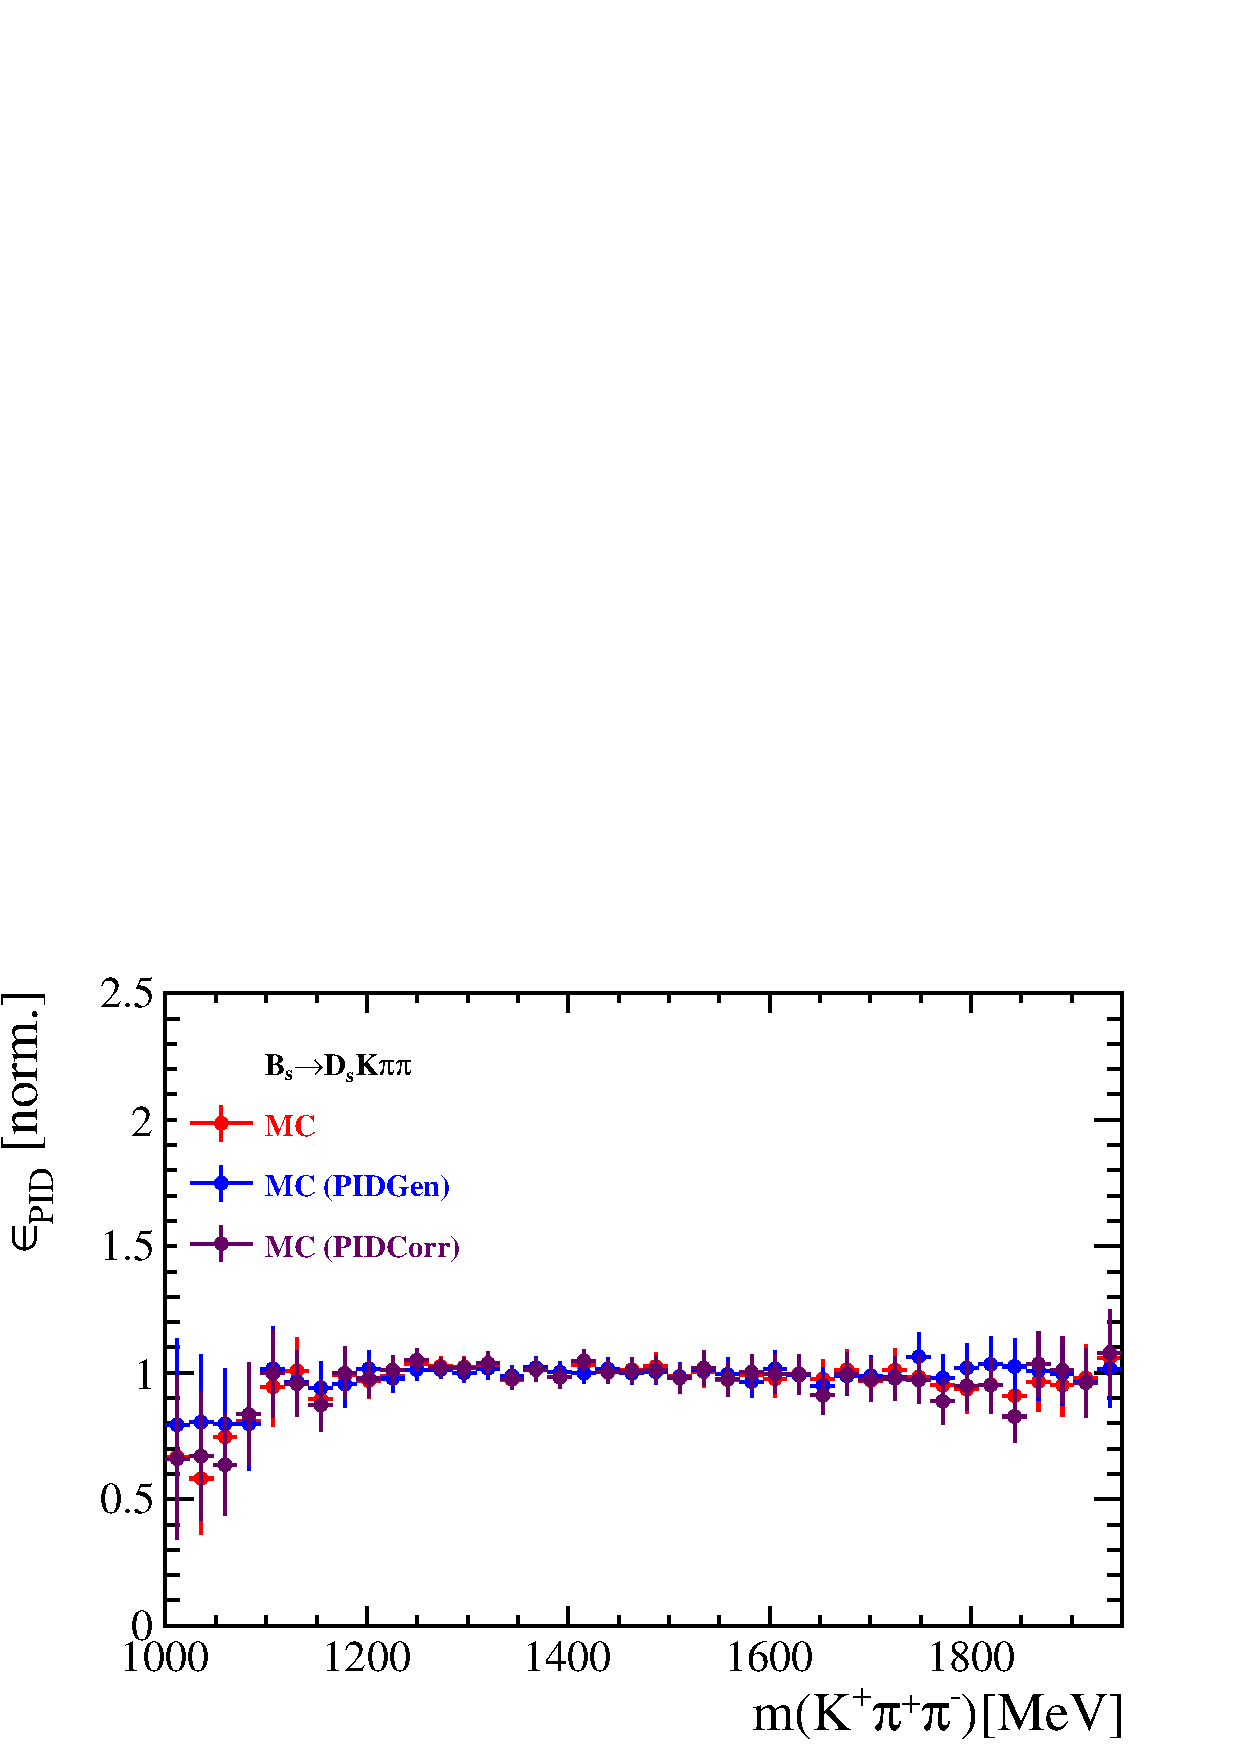
\includegraphics[height=!,width=0.32\textwidth]{figs/dataVsMC/signal_pid/eff_PID_Ds2KKpi_1_m_Kpipi.pdf}
%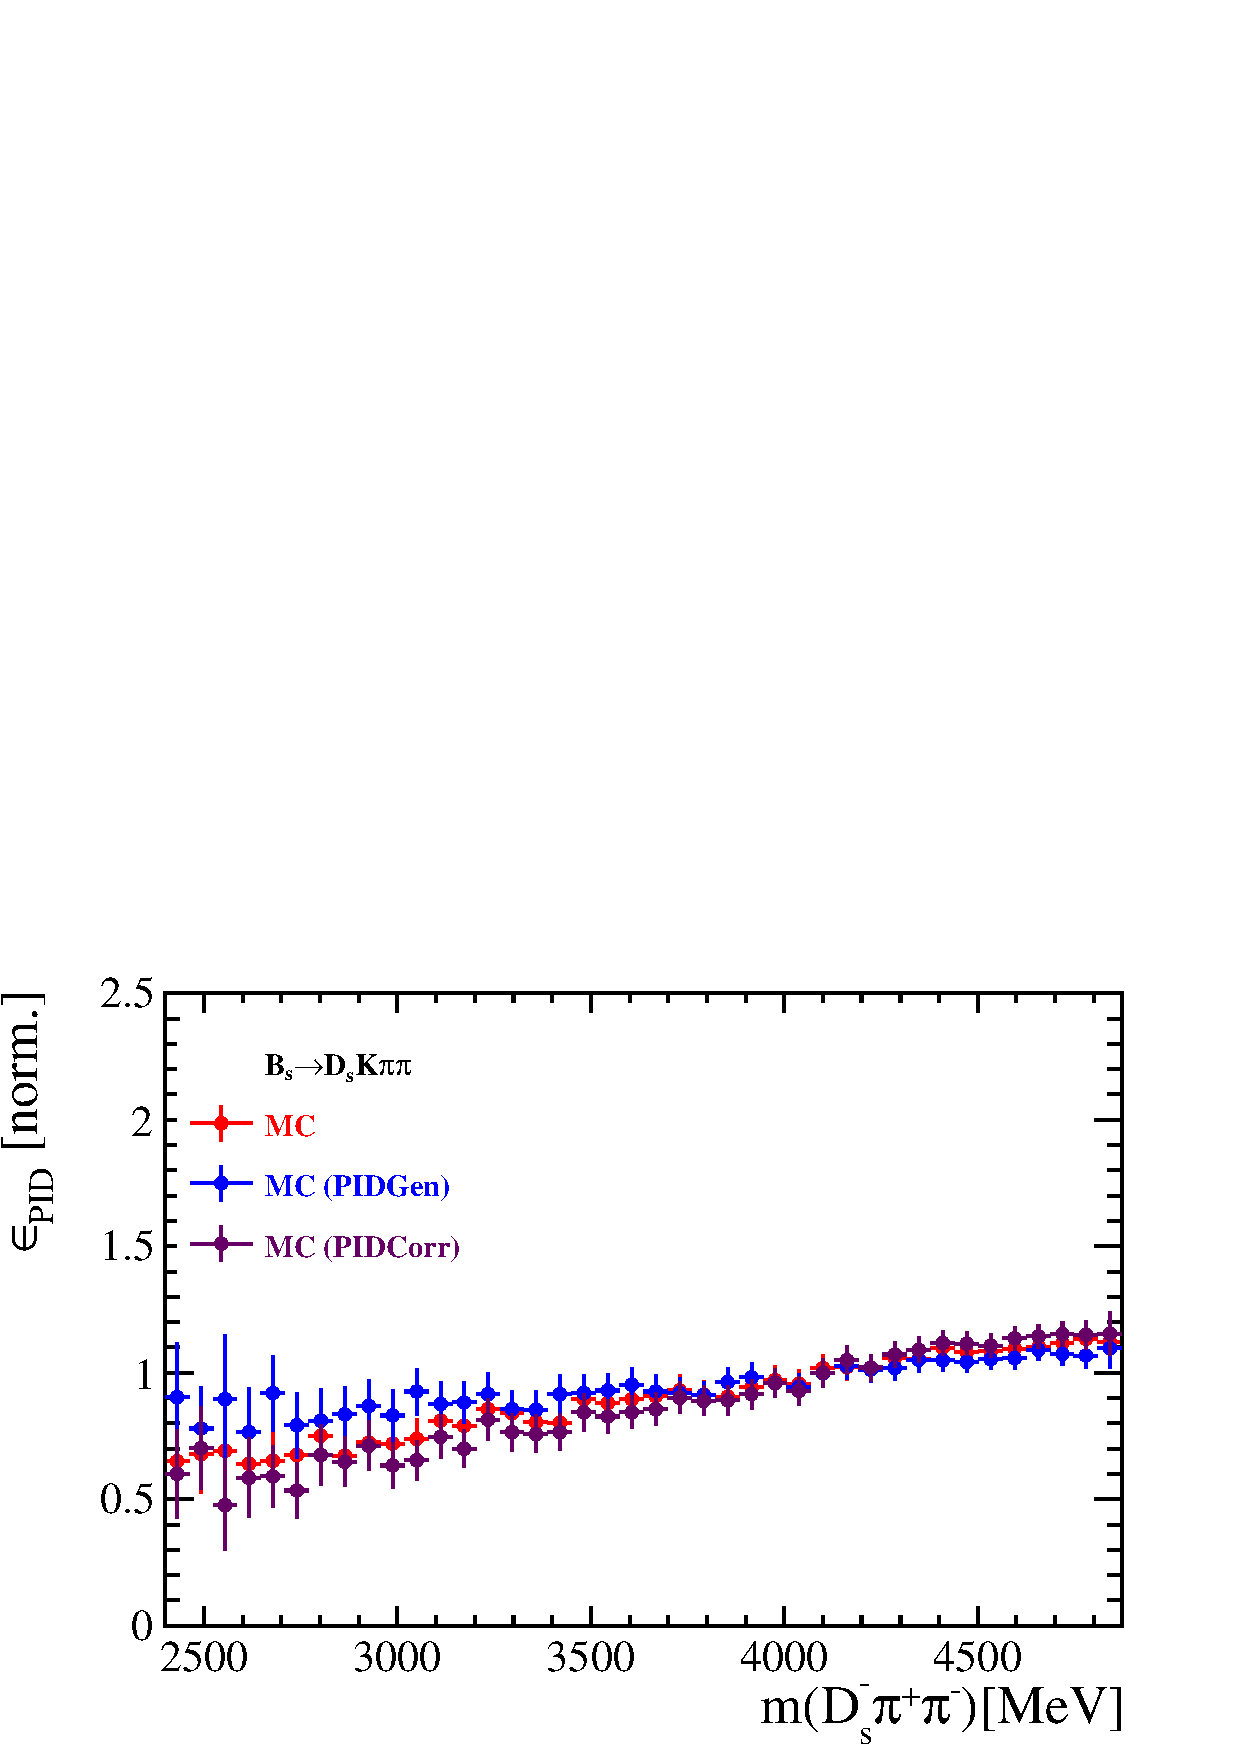
\includegraphics[height=!,width=0.32\textwidth]{figs/dataVsMC/signal_pid/eff_PID_Ds2KKpi_1_m_Dspipi.pdf}
%
%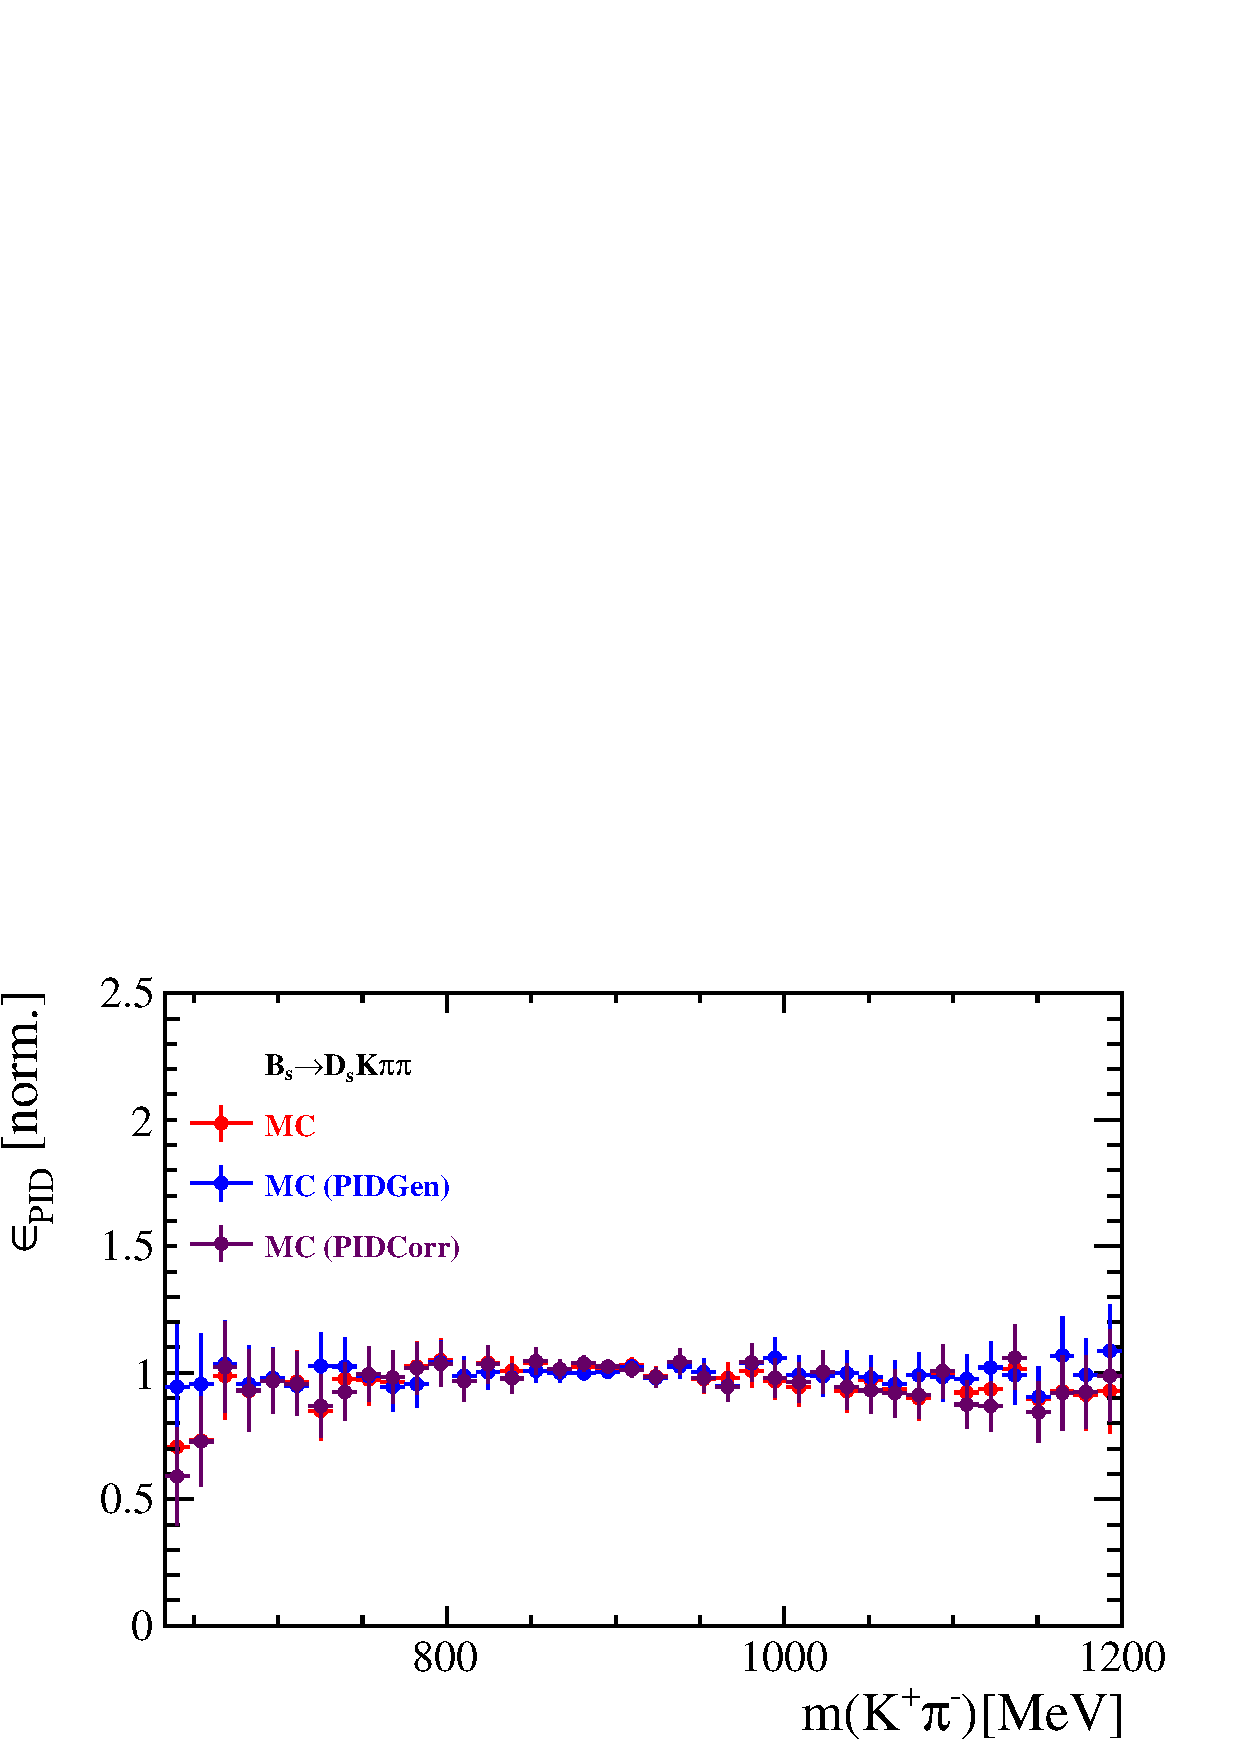
\includegraphics[height=!,width=0.32\textwidth]{figs/dataVsMC/signal_pid/eff_PID_Ds2KKpi_1_m_Kpi.pdf}
%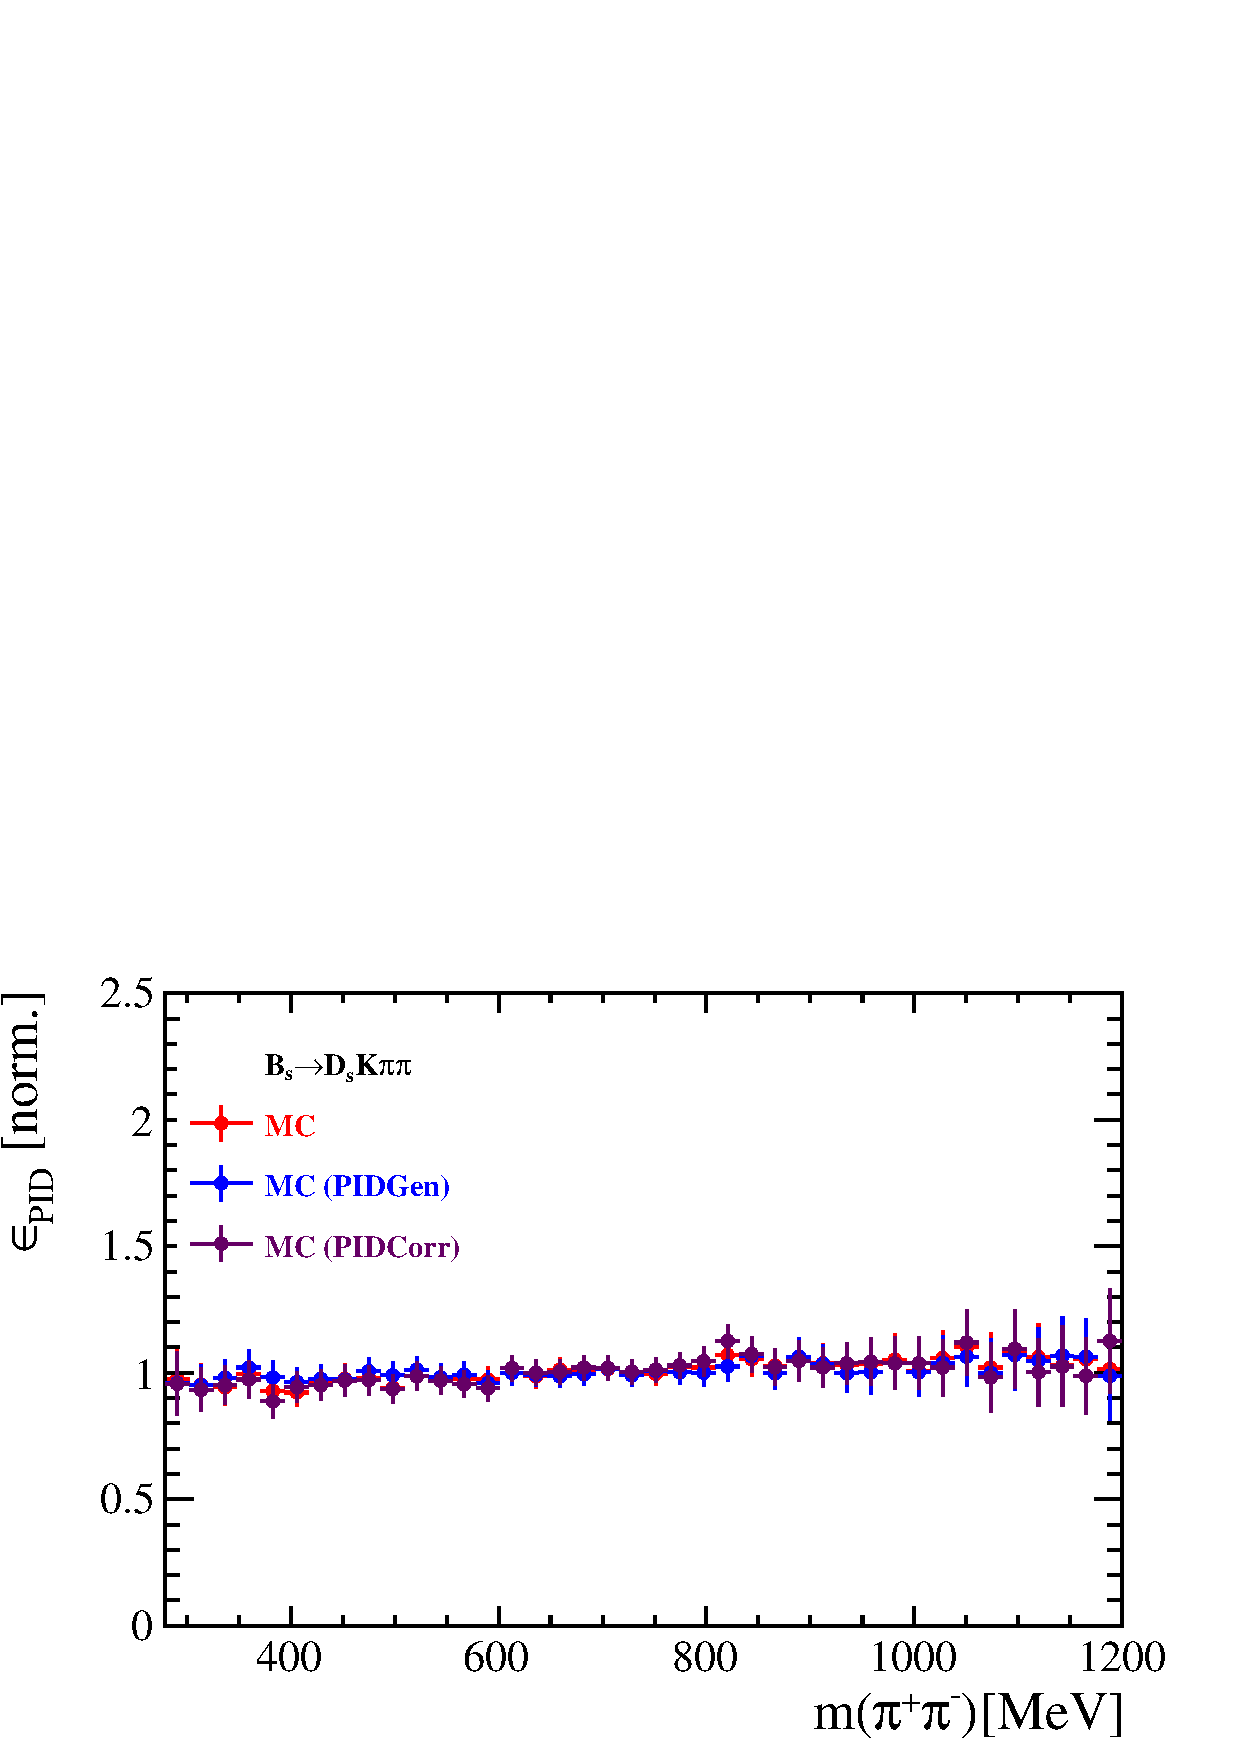
\includegraphics[height=!,width=0.32\textwidth]{figs/dataVsMC/signal_pid/eff_PID_Ds2KKpi_1_m_pipi.pdf}
%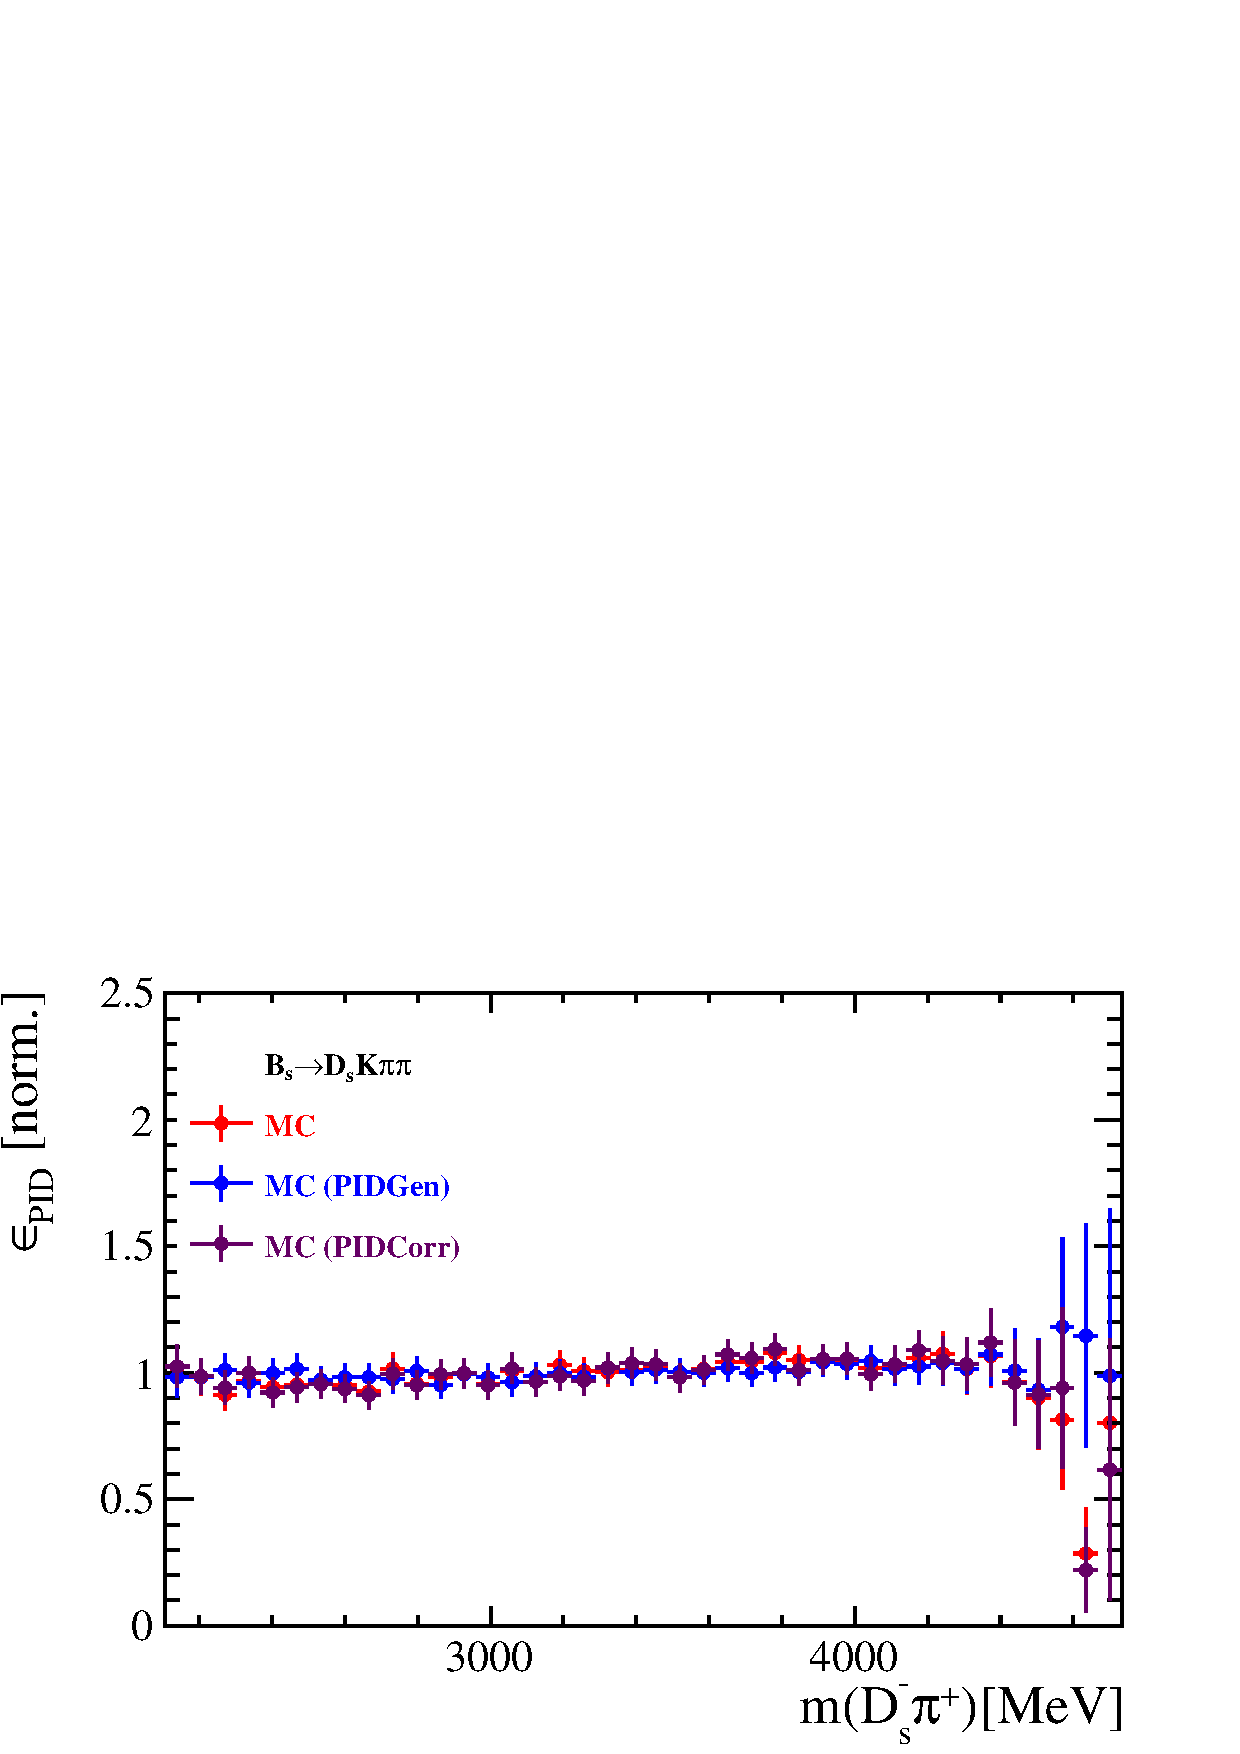
\includegraphics[height=!,width=0.32\textwidth]{figs/dataVsMC/signal_pid/eff_PID_Ds2KKpi_1_m_Dspi.pdf}
%\caption{}
%\label{fig:}
%\end{figure}
%
%
%\clearpage
%\subsubsection{BDT efficiencies}
%
%\begin{figure}[h]
%\includegraphics[height=!,width=0.32\textwidth]{figs/dataVsMC/signal_bdt/eff_Ds2KKpi_1_Bs_DTF_TAU.pdf}
%\includegraphics[height=!,width=0.32\textwidth]{figs/dataVsMC/signal_bdt/eff_Ds2KKpi_1_m_Kpipi.pdf}
%\includegraphics[height=!,width=0.32\textwidth]{figs/dataVsMC/signal_bdt/eff_Ds2KKpi_1_m_Dspipi.pdf}
%
%\includegraphics[height=!,width=0.32\textwidth]{figs/dataVsMC/signal_bdt/eff_Ds2KKpi_1_m_Kpi.pdf}
%\includegraphics[height=!,width=0.32\textwidth]{figs/dataVsMC/signal_bdt/eff_Ds2KKpi_1_m_pipi.pdf}
%\includegraphics[height=!,width=0.32\textwidth]{figs/dataVsMC/signal_bdt/eff_Ds2KKpi_1_m_Dspi.pdf}
%\caption{}
%\label{fig:}
%\end{figure}
%
%
%\begin{figure}[h]
%\includegraphics[height=!,width=0.32\textwidth]{figs/dataVsMC/signal_bdt_scan/eff_Ds2KKpi_1_Bs_DTF_TAU.pdf}
%\includegraphics[height=!,width=0.32\textwidth]{figs/dataVsMC/signal_bdt_scan/eff_Ds2KKpi_1_m_Kpipi.pdf}
%\includegraphics[height=!,width=0.32\textwidth]{figs/dataVsMC/signal_bdt_scan/eff_Ds2KKpi_1_m_Dspipi.pdf}
%
%\includegraphics[height=!,width=0.32\textwidth]{figs/dataVsMC/signal_bdt_scan/eff_Ds2KKpi_1_m_Kpi.pdf}
%\includegraphics[height=!,width=0.32\textwidth]{figs/dataVsMC/signal_bdt_scan/eff_Ds2KKpi_1_m_pipi.pdf}
%\includegraphics[height=!,width=0.32\textwidth]{figs/dataVsMC/signal_bdt_scan/eff_Ds2KKpi_1_m_Dspi.pdf}
%\caption{}
%\label{fig:}
%\end{figure}
%
%
%\clearpage
%\subsubsection{Tracking efficiencies}

\clearpage

\subsection{Decay-time acceptance}
\label{sec:timeAcceptance}
The decay-time distribution of the $\Bs$ mesons is sculpted due to the geometry of the LHCb detector and the applied selection cuts, which are described in Section \ref{sec:Selection}.
In particular, any requirement on the flight distance, the impact parameter or the direction angle (DIRA) of the $\Bs$ mesons, as well as the direct cut on the proper-time, will lead to a decay-time dependent efficiency $\epsilon(t)$. 

%This efficiency will distort the theoretically expected, time-dependent decay rate
%\begin{equation}
%\frac{\Gamma(t)^{observed}}{dt} = \frac{\Gamma(t)^{theory}}{dt} \cdot \epsilon(t),
%\label{eq:DecRateAcc}
%\end{equation} 
%and has to be modelled correctly, in order to describe the observed decay rate. 

We use our control channel for this measurement, because for $\Bs\to\Ds\kaon\pion\pion$ decays the decay-time acceptance is correlated with the \CP-observables which we aim to measure. Therefore, floating the \CP-observables and the acceptance shape at the same time is not possible. 
Hence, a fit to the decay-time distribution of $\Bs\to\Ds\pion\pion\pion$ candidates is performed and the obtained acceptance shape is corrected by the difference in shape found for the $\Bs\to\Ds\kaon\pion\pion$ and $\Bs\to\Ds\pion\pion\pion$ MC. \newline
A PDF of the form

\begin{equation}
\mathcal{P}(t) = \left[ e^{\Gamma_{s}t}\cdot \text{cosh}\left(\frac{\Delta\Gamma_{s} \, t^\prime}{2}\right) \times \mathcal{R}(t - t^{'})\right] \cdot \epsilon(t),
\label{eq:AccPDF}
\end{equation}

is fit to the decay time distribution of $\Bs\to\Ds\pion\pion\pion$ candidates in data. 
Since the fit is performed untagged, the PDF shown in Eq. \ref{eq:AccPDF} contains no terms proportional to $\dms$. 
The values for $\Gamma_{s}$ and $\Delta\Gamma_{s}$ are fixed to the latest HFAG results \cite{HFAG}. 
The decay-time acceptance $\epsilon(t^{'}, \vec{\lambda})$ is modelled using the sum of cubic polynomials $v_{i}(t)$, so called Splines \cite{Karbach:2014qba}. 
The polynomials are parametrised by so-called knots which determine their boundaries. Knots can be set across the fitted distribution to account for local changes in the acceptance shape.
Using more knots is equivalent to using more base splines which are defined on a smaller sub-range. 
In total, $n+2$ base splines $v_{i}(t)$ are needed to describe an acceptance shape which is parametrised using $n$ knots.\newline
For fits shown in the following, the knots have been placed at $t = [0.5, 1.0, 1.5, 2.0, 3.0, 9.5] ps$. To accommodate these 6 knot positions, 8 basic splines $v_{i}$, $i = [1,...,8]$ are used.
Since a rapid change of the decay time acceptance at low decay times due to the turn-on effect generated by the lifetime and other selection cuts is expected, more knots are placed in that regime.
At higher decay times we expect linear behavior, with a possible small effect due to the VELO reconstruction. Therefore fewer knots are used. 
Furthermore, $v_{7}$ is fixed to 1 in order to normalize the overall acceptance function. To stabilise the last spline, $v_{8}$ is fixed by a linear extrapolation from the two previous splines:

\begin{equation}   
v_{N} = v_{N-1} + \frac{v_{N-2} - v_{N-1}}{t_{N-2} - t_{N-1}} \cdot (t_{N} - t_{N-1}).
\label{eq:SplineExtra}
\end{equation}

Here, $N=8$ and $t_{N-1}$ corresponds to the knot position associated with $v_{N-1}$. 

\clearpage

\subsubsection{Comparison of acceptance in subsamples}
\label{subsec: AccComparison}

It is possible that the decay-time dependent efficiency deviates in different subsamples of our data. 
In particular, the acceptance could differentiate in subsamples with different final state kinematics, such as the run I \& run II sample, the various $\Ds$ final states and the ways an event is triggered at the L0 stage.
To investigate possible deviations, the full selected $\Bs\to\Ds\pion\pion\pion$ sample is split into subsamples according to the categories mentioned above (run, $\Ds$ state, L0 trigger). 
For each subsample, the fit procedure described at the beginning of this chapter, using the pdf given by Eq. \ref{eq:AccPDF}, is repeated and the obtained values for the spline coefficients  $v_{i}$ are compared.
Figure \ref{fig:AccCompDs} shows the comparison of the obtained spline coefficients for the different $\Ds$ final states.

%\begin{figure}[h]
%\includegraphics[height=!,width=\textwidth]{figs/Acceptance/adaptive_N4/timeAcc_combined_by_DsFinalState.pdf}
%\caption{Comparison of the spline coefficients obtained from time-dependent fits to the $\Bs\to\Ds\pion\pion\pion$ subsamples of different $\Ds$ final states. 
%The comparison of one particular $\Ds$ state against all other states is shown.}
%\label{fig:AccCompDs}
%\end{figure}

\begin{figure}[h]
\includegraphics[height=!,width=0.49\textwidth]{figs/Acceptance/timeAcc_comparison_by_year_t1_adaptive_N4.pdf}
\includegraphics[height=!,width=0.49\textwidth]{figs/Acceptance/timeAcc_comparison_by_run_adaptive_N4.pdf}

\includegraphics[height=!,width=0.49\textwidth]{figs/Acceptance/timeAcc_comparison_by_DsFinalState_mod_adaptive_N4.pdf}
\includegraphics[height=!,width=0.49\textwidth]{figs/Acceptance/timeAcc_comparison_by_trigger_adaptive_N4.pdf}
\caption{Comparison of the spline coefficients obtained from time-dependent fits to the $\Bs\to\Ds\pion\pion\pion$ subsamples of (left) the different runs and (right) L0 trigger categories.}
\label{fig:AccCompRunTrig}
\end{figure}

Investigating the obtained spline coefficients from different $\Ds$ final states, 
good agreement is observed between all four channels and no need to distinguish between different final states in the time-dependent amplitude fit is found. \newline
The comparison between spline coefficients for the different runs and L0 trigger categories is shown in Figure \ref{fig:AccCompRunTrig}.

Significant deviations between spline coefficients obtained from the two different runs and L0 trigger categories can be observed. 
The deviations are most pronounced in the $(0-5) \ps$ region, where the majority of statistics is found. 
Therefore, the time-dependent efficiency has to be treated separately for the runs and L0 categories. 
This is achieved by implementing a simultaneous fit, where the acceptance description is allowed to vary in the subsamples.   



\clearpage
\subsubsection{Results}

The nominal fit to $\Bs\to\Ds\pion\pion\pion$ data using this configuration is shown in Figure \ref{fig:accFit}. 
Note that the normalization of the splines in the following figures is not in scale.
The fit parameters obtained from the described fits to data and simulation are summarised in Table \ref{table:splines}.
%
%\begin{figure}[h]
%\includegraphics[height=!,width=0.49\textwidth]{figs/Acceptance/adaptive_N4/timeAccRatioFit_norm_combined.pdf}
%\includegraphics[height=!,width=0.49\textwidth]{figs/Acceptance/adaptive_N4/timeAccRatioFit_norm_mc_combined.pdf}
%\includegraphics[height=!,width=0.49\textwidth]{figs/Acceptance/adaptive_N4/timeAccRatioFit_signal_B0_combined.pdf}
%\includegraphics[height=!,width=0.49\textwidth]{figs/Acceptance/adaptive_N4/timeAccRatioFit_signal_mc_combined.pdf}
%\caption{The red line shows the spline function describing the acceptance and the blue line depicts the total fit function.}
%\label{fig:accFit}
%\end{figure}
%\begin{table}[h]
\centering
\caption{Summary of the obtained parameters from the acceptance fit (run == 1).} 
\begin{tabular}{l l l l l}
\hline
\hline
Knot position & Coefficient & $\Bs\to\Ds\kaon\pion\pion$ data & $\Bs\to\Ds\kaon\pion\pion$ MC & Ratio \\
\hline
0.4 & $v_{0}$ & 0.474 $\pm$ 0.023 & 0.492 $\pm$ 0.015 & 0.978 $\pm$ 0.045\\
0.8 & $v_{1}$ & 0.716 $\pm$ 0.036 & 0.729 $\pm$ 0.023 & 0.925 $\pm$ 0.047\\
1.6 & $v_{2}$ & 0.882 $\pm$ 0.062 & 0.926 $\pm$ 0.040 & 1.013 $\pm$ 0.064\\
2.5 & $v_{3}$ & 1.112 $\pm$ 0.030 & 1.101 $\pm$ 0.022 & 0.963 $\pm$ 0.033\\
6.5 & $v_{4}$ & 1.000 $\pm$ 0.000 & 1.000 $\pm$ 0.000 & 1.000 $\pm$ 0.000\\
10.0 & $v_{5}$ & 0.902 $\pm$ 0.000 & 0.911 $\pm$ 0.000 & 1.032 $\pm$ 0.000\\
\hline
\hline
\end{tabular}
\label{table:splines}
\end{table}


\clearpage
\begin{table}[hp!]
\centering
\small
\caption{Time acceptance parameters for events in category [\textsf{Run-I},\textsf{L0-TOS}].}
\begin{tabular}{c c c c c}
\hline
\hline
Knot position & Coefficient & $\Bs\to\Ds\kaon\pion\pion$ data & $\Bs\to\Ds\kaon\pion\pion$ MC & Ratio \\
\hline
0.4 & $v_{0}$ & 0.576 $\pm$ 0.021 & 0.537 $\pm$ 0.017 & 1.005 $\pm$ 0.051\\
0.8 & $v_{1}$ & 0.841 $\pm$ 0.024 & 0.788 $\pm$ 0.026 & 0.894 $\pm$ 0.040\\
1.6 & $v_{2}$ & 0.845 $\pm$ 0.068 & 0.914 $\pm$ 0.047 & 1.044 $\pm$ 0.074\\
2.5 & $v_{3}$ & 1.113 $\pm$ 0.040 & 1.107 $\pm$ 0.028 & 0.956 $\pm$ 0.043\\
6.5 & $v_{4}$ &  1.0 (fixed) & 1.0 (fixed) & 1.0 (fixed)\\
10.0 & $v_{5}$ & 0.901 (interpolated) & 0.907 (interpolated) & 1.038 (interpolated) \\
\hline
\hline
\end{tabular}
\label{table:splines}
\end{table}
\begin{table}[hp!]
\centering
\small
\caption{Time acceptance parameters for events in category [\textsf{Run-I},\textsf{L0-TIS}].}
\begin{tabular}{c c c c c}
\hline
\hline
Knot position & Coefficient & $\Bs\to\Ds\kaon\pion\pion$ data & $\Bs\to\Ds\kaon\pion\pion$ MC & Ratio \\
\hline
0.4 & $v_{0}$ & 0.372 $\pm$ 0.036 & 0.402 $\pm$ 0.021 & 1.046 $\pm$ 0.099\\
0.8 & $v_{1}$ & 0.598 $\pm$ 0.057 & 0.640 $\pm$ 0.034 & 0.898 $\pm$ 0.075\\
1.6 & $v_{2}$ & 0.917 $\pm$ 0.089 & 0.982 $\pm$ 0.057 & 0.905 $\pm$ 0.080\\
2.5 & $v_{3}$ & 1.091 $\pm$ 0.053 & 1.077 $\pm$ 0.035 & 1.007 $\pm$ 0.051\\
6.5 & $v_{4}$ &  1.0 (fixed) & 1.0 (fixed) & 1.0 (fixed)\\
10.0 & $v_{5}$ & 0.921 (interpolated) & 0.932 (interpolated) & 0.994 (interpolated) \\
\hline
\hline
\end{tabular}
\label{table:splines}
\end{table}
\begin{tabular}{c c c c c}
\hline
\hline
Knot position & Coefficient & $\Bs\to\Ds\kaon\pion\pion$ data & $\Bs\to\Ds\kaon\pion\pion$ MC & Ratio \\
\hline
0.4 & $v_{0}$ & 0.285 $\pm$ 0.009 & 0.368 $\pm$ 0.005 & 1.023 $\pm$ 0.020\\
0.5 & $v_{1}$ & 0.663 $\pm$ 0.017 & 0.749 $\pm$ 0.009 & 0.911 $\pm$ 0.016\\
1.4 & $v_{2}$ & 0.856 $\pm$ 0.025 & 0.893 $\pm$ 0.012 & 1.016 $\pm$ 0.019\\
2.5 & $v_{3}$ & 1.060 $\pm$ 0.017 & 1.071 $\pm$ 0.008 & 0.996 $\pm$ 0.013\\
6.5 & $v_{4}$ &  1.0 (fixed) & 1.0 (fixed) & 1.0 (fixed)\\
10.0 & $v_{5}$ & 0.948 (interpolated) & 0.938 (interpolated) & 1.004 (interpolated) \\
\hline
\hline
\end{tabular}

\begin{tabular}{c c c c c}
\hline
\hline
Knot position & Coefficient & $\Bs\to\Ds\kaon\pion\pion$ data & $\Bs\to\Ds\kaon\pion\pion$ MC & Ratio \\
\hline
0.4 & $v_{0}$ & 0.121 $\pm$ 0.006 & 0.176 $\pm$ 0.003 & 0.982 $\pm$ 0.032\\
0.5 & $v_{1}$ & 0.414 $\pm$ 0.014 & 0.479 $\pm$ 0.008 & 0.952 $\pm$ 0.023\\
1.4 & $v_{2}$ & 0.746 $\pm$ 0.023 & 0.784 $\pm$ 0.013 & 0.967 $\pm$ 0.024\\
2.5 & $v_{3}$ & 1.053 $\pm$ 0.018 & 1.041 $\pm$ 0.010 & 0.991 $\pm$ 0.015\\
6.5 & $v_{4}$ &  1.0 (fixed) & 1.0 (fixed) & 1.0 (fixed)\\
10.0 & $v_{5}$ & 0.953 (interpolated) & 0.964 (interpolated) & 1.008 (interpolated) \\
\hline
\hline
\end{tabular}


\clearpage
\begin{figure}[h]
\includegraphics[height=!,width=0.49\textwidth]{figs/Acceptance/adaptive_N4/timeAccRatioFit_norm_Run1_t0.pdf}
\includegraphics[height=!,width=0.49\textwidth]{figs/Acceptance/adaptive_N4/timeAccRatioFit_norm_mc_Run1_t0.pdf}
\includegraphics[height=!,width=0.49\textwidth]{figs/Acceptance/adaptive_N4/timeAccRatioFit_signal_B0_Run1_t0.pdf}
\includegraphics[height=!,width=0.49\textwidth]{figs/Acceptance/adaptive_N4/timeAccRatioFit_signal_mc_Run1_t0.pdf}
\caption{}
\label{fig:}
\includegraphics[height=!,width=0.49\textwidth]{figs/Acceptance/adaptive_N4/timeAccRatioFit_norm_Run1_t1.pdf}
\includegraphics[height=!,width=0.49\textwidth]{figs/Acceptance/adaptive_N4/timeAccRatioFit_norm_mc_Run1_t1.pdf}
\includegraphics[height=!,width=0.49\textwidth]{figs/Acceptance/adaptive_N4/timeAccRatioFit_signal_B0_Run1_t1.pdf}
\includegraphics[height=!,width=0.49\textwidth]{figs/Acceptance/adaptive_N4/timeAccRatioFit_signal_mc_Run1_t1.pdf}
\caption{}
\label{fig:}
\end{figure}

\clearpage
\begin{figure}[h]
\includegraphics[height=!,width=0.49\textwidth]{figs/Acceptance/adaptive_N4/timeAccRatioFit_norm_Run2_t0.pdf}
\includegraphics[height=!,width=0.49\textwidth]{figs/Acceptance/adaptive_N4/timeAccRatioFit_norm_mc_Run2_t0.pdf}
\includegraphics[height=!,width=0.49\textwidth]{figs/Acceptance/adaptive_N4/timeAccRatioFit_signal_B0_Run2_t0.pdf}
\includegraphics[height=!,width=0.49\textwidth]{figs/Acceptance/adaptive_N4/timeAccRatioFit_signal_mc_Run2_t0.pdf}
\caption{}
\label{fig:}
\includegraphics[height=!,width=0.49\textwidth]{figs/Acceptance/adaptive_N4/timeAccRatioFit_norm_Run2_t1.pdf}
\includegraphics[height=!,width=0.49\textwidth]{figs/Acceptance/adaptive_N4/timeAccRatioFit_norm_mc_Run2_t1.pdf}
\includegraphics[height=!,width=0.49\textwidth]{figs/Acceptance/adaptive_N4/timeAccRatioFit_signal_B0_Run2_t1.pdf}
\includegraphics[height=!,width=0.49\textwidth]{figs/Acceptance/adaptive_N4/timeAccRatioFit_signal_mc_Run2_t1.pdf}
\caption{}
\label{fig:}
\end{figure}

\clearpage
\subsection{Phasespace acceptance}
\label{sec:phasespaceAcceptance}

\pretextcomment{Disclaimer: ...}

In general, the signal PDF for events tagged as $\Dz \to h^+ h^- \pip \pim$ is given by
\begin{equation}
	\mathcal P_{\rm Sig}(\phsPoint) %= \frac{ \vert \mathcal M(X) \vert^{2} \, \phi_{4}(X) }{\int  \vert \mathcal M(X) \vert^{2} \, \phi_{4}(X) \, \text{d}X} 
	=  
	\frac{ [(1-w)\left\vert   A_{\Dz}(\phsPoint) \right\vert^{2} + w \, \left\vert    A_{\Dzb}(\phsPoint) \right\vert^{2} ]\,\epsilon_{\rm Sig}(\phsPoint) \, \phsd(\phsPoint) }
	{\int [\left\vert  A_{\Dz}(\phsPoint) \right\vert^{2} + \left\vert    A_{\Dzb}(\phsPoint) \right\vert^{2} ]\, \epsilon_{\rm Sig}(\phsPoint) \, \text{d}\Phi_{4} } , 
\label{eq:sigPDF}
\end{equation}
where
$\epsilon_{\rm Sig}(\phsPoint)$ is the phase-space efficiency. 


Note that the efficiency in the numerator appears as an additive constant in the $\log {\cal L}$ that does not depend on any fit parameters such that it can be ignored.
However, the efficiency function still enters via the normalization integrals. 
These normalization terms are determined numerically by a MC integration technique.
For this purpose, we use simulated events generated according to a preliminary model, pass them 
through the full detector simulation and apply the same selection criteria as for data 
in order to perform the MC integrals.
For example, the first integral in \eqnPRDref{eq:sigPDF} can be approximated as 
\begin{equation}
	\int \left\vert   A_{\Dz}(\phsPoint) \right\vert^{2} \, \epsilon_{\rm Sig}(\phsPoint) \, \text{d}\Phi_{4}   \approx 
	\frac{1}{N_{\rm MC}} \, \sum_{k}^{N_{\rm MC}}    \frac{\left\vert   A_{\Dz}(\bold{x_{k}}) \right\vert^{2}}
	{\left\vert A_{\Dz}^{\prime}(\bold{x_{k}}) \right\vert^{2}}
\end{equation}
where $A_{\Dz}^{\prime}$ labels the preliminary amplitude model and
$x_{k}$ is the $k$-th MC event. As a result, the efficiency can be included in the amplitude fit without explicitly modeling it.
For $\Dz \to \pi^+ \pi^- \pip \pim$, we use a sample of $N_{\rm MC}  = 600 000$  MC events to 
ensure that the uncertainty on the integral is less than $0.5 \%$.



\begin{figure}[h]
\centering
\includegraphics[height=!,width=0.8\textwidth]{figs/AcceptancePhspBDT/variables_id_c1.pdf}
\caption{}
\label{fig:}
\end{figure}


\begin{figure}[h]
\centering
\includegraphics[height=!,width=0.49\textwidth]{figs/AcceptancePhspBDT/BDTG.pdf}
\includegraphics[height=!,width=0.49\textwidth]{figs/AcceptancePhspBDT/eff.pdf}
\caption{}
\label{fig:}
\end{figure}

\begin{figure}[h]
\centering
\includegraphics[height=!,width=0.32\textwidth]{figs/AcceptancePhspBDT/eff_Kpipi.pdf}
\includegraphics[height=!,width=0.32\textwidth]{figs/AcceptancePhspBDT/eff_Kpi.pdf}
\includegraphics[height=!,width=0.32\textwidth]{figs/AcceptancePhspBDT/eff_pipi.pdf}

\includegraphics[height=!,width=0.32\textwidth]{figs/AcceptancePhspBDT/eff_Dspipi.pdf}
\includegraphics[height=!,width=0.32\textwidth]{figs/AcceptancePhspBDT/eff_Dspi.pdf}

\includegraphics[height=!,width=0.32\textwidth]{figs/AcceptancePhspBDT/eff_cosTheta_Kpi.pdf}
\includegraphics[height=!,width=0.32\textwidth]{figs/AcceptancePhspBDT/eff_cosTheta_Dspi.pdf}
\includegraphics[height=!,width=0.32\textwidth]{figs/AcceptancePhspBDT/eff_phi_Kpi_Dspi.pdf}

\caption{}
\label{fig:}
\end{figure}
